\chapter{中厚板剪切自锁问题}
本章针对中厚板剪切自锁问题,提出了有限元无网格混合离散分析方法最优约束比例。首先介绍了中厚板问题的混合离散过程,
其次对比中厚板问题的最优约束比例和传统约束比例。最后通过算例验证该方法的计算精度。

\section{剪切自锁问题}    
\subsection{罚函数法}
考虑如图\ref{mindlin_picture}所示中厚板,其中中板厚为$h$,$\Omega$为板中面。在Mindlin假设下,中厚板考虑横向剪切变形,相应的混合控制方程由下式给出:
\begin{equation}\label{strong_mindlin}
    \begin{cases}
        M_{\alpha\beta,\beta} - Q_\alpha = 0 & \textrm{in}\; \Omega \\
        Q_{\alpha,\alpha} + \bar q = 0 & \textrm{in}\; \Omega \\    Q_\alpha n_\alpha = \bar Q & \textrm{on}\; \Gamma_Q \\
        M_{\alpha\beta} n_\beta = \bar M_\alpha & \textrm{on}\; \Gamma_M \\
        \varphi_\alpha = \bar \varphi_\alpha & \textrm{on}\; \Gamma_\varphi \\
        w = \bar w & \textrm{on}\; \Gamma_w \\
    \end{cases}
\end{equation}
\begin{figure}
    \centering 
        \includegraphics[scale=0.5]{figures/shearlocking/Mindlinplate.png}
        \caption{中厚板运动学及边界条件}\label{mindlin_picture}
\end{figure}
式中,$M_{\alpha \beta}$ 可表示弯矩张量$\pmb{M}$ 的弯曲或扭转部分的分量,$\bar{q}$ 为垂直于板中面的分布荷载;
$\Gamma_w$和$\Gamma_\varphi$为本质边界条件,$\bar{w}$和$\bar{\varphi}_\alpha$分别为本质边界条件上给定的挠度和转角;
$\Gamma_Q$ 和$\Gamma_M$ 为自然边界条件,$\bar Q$和$\bar{M}_{\alpha}$ 为自然边界上的等效剪力和法向弯矩;
$n_\alpha$为边界上外法线方向$\pmb{n}$的分量。


在平面应力假设下,当中厚板为线弹性各同向性材料时,其本构关系为:
\begin{equation} 
    \begin{split}
    M_{\alpha \beta}=-\frac{h^3}{12}D_{\alpha \beta \gamma\eta}\kappa_{\gamma\eta}=\frac{h^3}{12}D_{\alpha \beta \gamma\eta}\varphi_{\gamma,\eta}
    \end{split}
\end{equation}
\begin{equation} 
    \begin{split}
    Q_{\alpha}=k\frac{Eh}{2(1+\nu)}\gamma_\beta=kGh(-\varphi_\beta+w_{,\beta})
    \end{split}
\end{equation}
其中$k$为剪切修正系数,$\kappa_{\alpha\beta}$为曲率张量$\pmb\kappa$的分量,$\gamma_\alpha$为剪切应变矢量$\pmb\gamma$的分量,表达式为:
\begin{equation} 
    \kappa_{\alpha\beta}=-\varphi_{\alpha,\beta},\quad\gamma_\alpha=-\varphi_\alpha+w_{,\alpha}
\end{equation}
其中$D_{\alpha \beta \gamma\eta}$为在平面应力假设下四阶弹性张量的分量,表达式为:
\begin{equation} 
    D_{\alpha \beta \gamma\eta}=\frac{E}{1-\nu^2}(\nu\delta_{\alpha\beta}\delta_{\gamma\eta}+\frac{1}{2}(1-\nu)(\delta_{\alpha\gamma}\delta_{\beta\eta}+\delta_{\alpha\eta}\delta_{\beta\gamma}))
\end{equation}

根据最小势能原理,强形式\eqref{strong_mindlin}所对应的势能泛函表达式为: 
\begin{equation}\label{potential_energy}
    \begin{split} 
        \Pi(w,\boldsymbol{\varphi})&=\frac{1}{2}\int_{\Omega}\kappa_{\alpha\beta}M_{\alpha\beta}d\Omega+\frac{1}{2}\int_{\Omega}\gamma_{\alpha}Q_{\alpha}d\Omega\\
        &+\int_{\Gamma_{M}}\varphi_{\alpha}{\bar{M}_{\alpha}}d\Gamma-\int_{\Gamma_{Q}}{w}\bar {Q}d\Gamma-\int_{\Omega} w\bar{q}d\Omega
    \end{split}
\end{equation}
对式\eqref{potential_energy}进行变分可得弱形式:
存在$(w,\varphi_{\alpha})\in V$,使
\begin{equation}\label{weak_penalty_mindlin}
    \begin{split} 
        &\int_{\Omega}\delta\kappa_{\alpha\beta}M_{\alpha\beta}d\Omega+\int_{\Omega}\delta\gamma_{\alpha}Q_{\alpha}d\Omega=\\
        &-\int_{\Gamma_{M}}\delta\varphi_{\alpha}{\bar{M}_{\alpha}}d\Gamma+\int_{\Gamma_{Q}}{\delta{w}}\bar {Q}d\Gamma+\int_{\Omega} \delta{w}\bar{q}d\Omega,\quad \forall(\delta w,\delta\varphi_{\alpha}) \in V
    \end{split}
\end{equation}

在传统有限元法中,整个影响域$\Omega$由一组具有节点$\{\boldsymbol x_I\}_{I=1}^{n_u}$的构造网格离散,其中$n_u$是节点的数量。
挠度$w$及其变分$\delta w $,转角$\varphi_\alpha$及其变分$\delta \varphi_\alpha $可通过$x_I$处的节点系数和形函数进行近似:
\begin{equation}
    w^h(\boldsymbol x) = \sum_{I=1}^{n_u} N_I(\boldsymbol x) w_I, \quad \delta w^h(\boldsymbol x) = \sum_{I=1}^{n_u} N_I(\boldsymbol x) \delta w_I
\end{equation}
\begin{equation}
    \varphi^h_{\alpha}(\boldsymbol x) = \sum_{I=1}^{n_u} N_I(\boldsymbol x) \varphi_{\alpha I}, \quad \delta \varphi^h(\boldsymbol x) = \sum_{I=1}^{n_u} N_I(\boldsymbol x) \delta \varphi_{\alpha I}
\end{equation}
其中,$N_I$为节点$x_I$处的形函数,和$w_I$和$\varphi_{\alpha I}$节点系数张量。
相应的近似曲率$\pmb\kappa$和近似剪切应变$\pmb\gamma$可表示为:
\begin{equation}
    \boldsymbol\kappa^h = 
    \begin{Bmatrix}
        \kappa^h_{11} \\ \kappa^h_{22} \\ 2\kappa^h_{12} 
    \end{Bmatrix} = -\sum_{I=1}^{n_u}
    \begin{bmatrix}
        0 & N_{I,1} & 0 \\ 0 & 0 & N_{I,2} \\ 0 & N_{I,2} & N_{I,1}
    \end{bmatrix}
    \begin{Bmatrix}
        w_I \\ \varphi_{1I} \\ \varphi_{2I}
    \end{Bmatrix} = - \sum_{I=1}^{n_u} \boldsymbol B^b_I \boldsymbol d_I
\end{equation}
\begin{equation}
    \boldsymbol\gamma^h = 
    \begin{Bmatrix}
        \gamma^h_1 \\ \gamma^h_2
    \end{Bmatrix} = \sum_{I=1}^{n_u}
    \begin{bmatrix}
        N_{I,1} & N_I & 0 \\
        N_{I,2} & 0 & N_I
    \end{bmatrix}
    \begin{Bmatrix}
        w_I \\ \varphi_{1I} \\ \varphi_{2I}
    \end{Bmatrix} = \sum_{I=1}^{n_u} \boldsymbol B^s_I \boldsymbol d_I
\end{equation}
\begin{equation}\label{kappa_h}
    \delta\boldsymbol\kappa^h = - \sum_{I=1}^{n_u} \boldsymbol B^b_I \delta\boldsymbol d_I ,\quad \delta\boldsymbol\gamma^h = \sum_{I=1}^{n_u} \boldsymbol B^s_I \delta\boldsymbol d_I
\end{equation}
将式\eqref{kappa_h}代入到弱形式\eqref{weak_penalty_mindlin}可得下列变分方程:
存在$(w^h,\boldsymbol{\varphi}^h_{\alpha})\in V_h$,使
\begin{equation}\label{ritz_penalty_mindlin}
    \begin{split} 
        &\int_{\Omega}\delta\kappa^h_{\alpha\beta}M_{\alpha\beta}d\Omega+\int_{\Omega}\delta\gamma^h_{\alpha}Q_{\alpha}d\Omega=\\
        &-\int_{\Gamma_{M}}\delta\varphi^h_{\alpha}{\bar{M}_{\alpha}}d\Gamma+\int_{\Gamma_{Q}}{\delta{w^h}}\bar {Q}d\Gamma+\int_{\Omega} \delta{w^h}\bar{q}d\Omega,\quad \forall(\delta w^h,\delta\varphi^h_{\alpha}) \in V_h
    \end{split}
\end{equation}

根据$\pmb\kappa^h$和$\pmb\gamma^h$的任意性,上述方程可简化为如下离散控制方程:
\begin{equation}
    (\boldsymbol K^b + \boldsymbol K^s) \boldsymbol d = \boldsymbol f
\end{equation}
其中弯曲刚度矩阵$\boldsymbol K^b$和剪切刚度矩阵$\boldsymbol K^s$是具有以下分量:
\begin{subequations}\label{stiffness_mindlin}
    \begin{alignat}{2}
    \label{stiffness_bending}
    \boldsymbol K^b_{IJ} = \frac{h^3}{12} \int_\Omega \boldsymbol B^{bT}_I \boldsymbol D \boldsymbol B^b_J d\Omega\\
    \label{stiffness_shear}
    \boldsymbol K^s_{IJ} = h \int_\Omega \boldsymbol B^{sT}_I kG \boldsymbol B^s_J d\Omega
    \end{alignat}
\end{subequations}
式中$\pmb{D}$为平面应力弹性矩阵,$\pmb{f}$为力矢量,其分量具有以下形式:
\begin{equation}
    \boldsymbol f_I = \int_{\Gamma_Q} N_I \bar{\boldsymbol Q} d\Gamma - \int_{\Gamma_M} N_I \bar{\boldsymbol M} d\Gamma + \int_\Omega N_I \bar{\boldsymbol q} d\Omega
\end{equation}
其中:
\begin{equation}
    \bar{\boldsymbol Q} =  
    \begin{Bmatrix}
        \bar Q \\ 0 \\ 0
    \end{Bmatrix},
        \bar{\boldsymbol M} =
    \begin{Bmatrix}
        0 \\ \bar M_1 \\ \bar M_2
    \end{Bmatrix},
        \bar{\boldsymbol q} =
    \begin{Bmatrix}
        \bar q \\ 0 \\ 0
    \end{Bmatrix}
\end{equation}

从式\eqref{stiffness_mindlin},对于考虑厚度方向变形的中厚板,当厚度$h$减少时,剪切刚度远大于弯曲刚度,使得板弯曲变形为$0$,而产生虚假的横向剪切应力。
由于这种情况,使用传统有限元法会产生严重的剪切锁定,就是所谓的剪切自锁。通过减少剪切刚度矩阵中积分点的数量,可以缓解剪切自锁。将数值积分代入式\eqref{ritz_penalty_mindlin}
\begin{equation}
    \int_{\Omega}\delta\gamma^h_{\alpha}Q_{\alpha}d\Omega \approx
    \sum_{C=1}^{n_e}\sum_{G=1}^{n_g} h \delta\gamma^h_{\alpha}(\boldsymbol x_G) kG \delta\gamma^h_{\alpha}(\boldsymbol x_G) w_G
\end{equation}
式\eqref{stiffness_shear}中的剪切刚度矩阵$\boldsymbol K^s$的分量可以改写为:
\begin{equation}
    \boldsymbol K^s_{IJ} \approx \bar{\boldsymbol K}^s_{IJ} = \sum_{C=1}^{n_e}\sum_{G=1}^{n_g} h\boldsymbol B^{sT}_I(\boldsymbol x_G) kG\boldsymbol B_J^s(\boldsymbol x_G) w_G
\end{equation}

\subsection{混合离散法}
为了缓解厚度减小引起的剪切自锁,引入与挠度和转角无关的剪切应力$\pmb{Q}$,根据最小势能原理,势能泛函的表达式可更改为:
\begin{equation}\label{potential_energy_mixed}
\begin{split} 
    \Pi(w,\boldsymbol{\varphi},\boldsymbol{Q})&=\int_{\bar\Omega}\frac{1}{2}\varepsilon_{ij}\sigma_{ij} d\Omega+\frac{1}{2}\int_{\Omega}Q_{\alpha}(\gamma_{\alpha}-\frac{Q_{\alpha}}{kGh})d\Omega-\int_{\Gamma^{t}} u_{i}t_{i}d\Gamma-\int_{\Omega} u_{i}b_{i}d\Omega\\
    &=\frac{1}{2}\int_{\Omega}(\kappa_{\alpha \beta}M_{\alpha \beta}+\gamma_{\alpha}Q_{\alpha})d\Omega+\frac{1}{2}\int_{\Omega}Q_{\alpha}(\gamma_{\alpha}-\frac{Q_{\alpha}}{kGh})d\Omega\\
    &+\int_{\Gamma_{M}}\pmb\varphi_{\alpha}{\bar{M}_{\alpha}}d\Gamma-\int_{\Gamma_{Q}}{w}\bar {Q}d\Gamma-\int_{\Omega} w\bar{q}d\Omega
\end{split}
\end{equation}
对式\eqref{potential_energy_mixed}进行变分可得弱形式:
\begin{equation} 
    \begin{split}
    &\delta\Pi(w,\boldsymbol\varphi,\boldsymbol{Q})\\
    &=\int_{\Omega}\delta\kappa_{\alpha \beta}M_{\alpha \beta}d\Omega+\frac{1}{2}\int_{\Omega}\delta\gamma_{\alpha}Q_{\alpha}d\Omega+\frac{1}{2}\int_{\Omega}\gamma_{\alpha}\delta{Q}_{\alpha}d\Omega+\frac{1}{2}\int_{\Omega}\delta\gamma_{\alpha}Q_{\alpha}d\Omega\\
    &+\frac{1}{2}\int_{\Omega}\gamma_{\alpha}\delta{Q}_{\alpha}d\Omega-\int_{\Omega}\frac{\delta{Q}_{\alpha}{Q}_{\alpha}}{kGh}d\Omega+\int_{\Gamma_{M}}\delta\varphi_{\alpha}{{\bar M}_{\alpha}}d\Gamma-\int_{\Gamma_{Q}}\delta{w}{\bar Q}d\Gamma+\int_{\Omega} \delta{w}\bar{q}d\Omega\\
    &=\int_{\Omega}\delta\kappa_{\alpha \beta}M_{\alpha \beta}d\Omega+\int_{\Omega}\delta\gamma_{\alpha}Q_{\alpha}d\Omega+\int_{\Omega}\gamma_{\alpha}\delta{Q}_{\alpha}d\Omega-\int_{\Omega}\frac{\delta{Q}_{\alpha}{Q}_{\alpha}}{kGh}d\Omega+\int_{\Gamma_{M}}\delta\varphi_{\alpha}{\boldsymbol{\bar M}_{\boldsymbol{\alpha}}}d\Gamma\\
    &-\int_{\Gamma_{Q}}\delta{w}{\bar Q}d\Gamma+\int_{\Omega} \delta{w}\bar{q}d\Omega\\
    &=0
    \end{split}
\end{equation}
由上式弱形式可以定义为:
存在$\boldsymbol u \in V$, $\boldsymbol p \in Q$,使
\begin{equation}
    \begin{aligned}
        a(\boldsymbol v, \boldsymbol u) + b(\boldsymbol v, \boldsymbol p) &= f(\boldsymbol v) \quad &\forall \boldsymbol v \in V \\
        b(\boldsymbol u, \boldsymbol q) &= \boldsymbol 0 \quad &\forall q \in Q
    \end{aligned}
\end{equation}
其中$\boldsymbol u=(w,\varphi_1,\varphi_2)$,具体表达式为:
\begin{equation}\label{mindlin_weak1}
    \int_{\Omega}\delta\kappa_{\alpha \beta}M_{\alpha \beta}d\Omega+\int_{\Omega}\delta\gamma_{\alpha}Q_{\alpha}d\Omega=\int_{\Gamma_{Q}}\delta{w}{\bar Q}d\Gamma-\int_{\Omega} \delta{w}\bar{q}d\Omega-\int_{\Gamma_{M}}\delta\varphi_{\alpha}{{\bar M}_{\alpha}}d\Gamma
\end{equation}
\begin{equation}\label{mindlin_weak2}
    \int_{\Omega}\gamma_{\alpha}\delta{Q}_{\alpha}d\Omega-\int_{\Omega}\frac{\delta{Q}_{\alpha}{Q}_{\alpha}}{kGh}d\Omega=0
\end{equation}
对挠度、转角和剪切应力采用混合离散的方式进行近似。近似剪切应力$Q_\alpha^h$可表示为:
\begin{equation}\label{Q_h}
    Q^h_\alpha(\boldsymbol x) = \sum_{K=1}^{n_q} N^q_K(\boldsymbol x) q_{\alpha K},\quad \delta Q^h_\alpha(\boldsymbol x) = \sum_{K=1}^{n_q} N^q_K(\boldsymbol x) \delta q_{\alpha K}
\end{equation}
其中$q_{\alpha K}$是节点系数,$N^q_K$是对应的形函数。相应的里兹-伽辽金变分方程如下:
存在$\boldsymbol u_h \in V_h$, $\boldsymbol p_h \in Q_h$使
\begin{equation}
    \begin{aligned}
        a(\boldsymbol v_h, \boldsymbol u_h) + b(\boldsymbol v_h, \boldsymbol p_h) &= f(\boldsymbol v_h) \quad &\forall \boldsymbol v_h \in V_h \\
        b(\boldsymbol u_h, \boldsymbol q_h) &= \boldsymbol 0 \quad &\forall \boldsymbol q_h \in Q_h
    \end{aligned}
\end{equation}
具体表达式为:
\begin{equation}\label{mindlin_ritz1}
    \int_{\Omega}\delta\kappa^h_{\alpha \beta}M_{\alpha \beta}d\Omega+\int_{\Omega}\delta\gamma^h_{\alpha}Q_{\alpha}d\Omega=\int_{\Gamma_{Q}}\delta{w_h}{\bar Q}d\Gamma-\int_{\Omega} \delta{w_h}\bar{q}d\Omega-\int_{\Gamma_{M}}\delta\varphi_{\alpha h}{{\bar M}_{\alpha}}d\Gamma
\end{equation}
\begin{equation}\label{mindlin_ritz2}
    \int_{\Omega}\gamma^h_{\alpha}\delta{Q}^h_{\alpha}d\Omega-\int_{\Omega}\frac{\delta{Q}^h_{\alpha}{Q}^h_{\alpha}}{kGh}d\Omega=0
\end{equation}

根据$\boldsymbol\kappa^h$、$\boldsymbol\gamma^h$和$\boldsymbol Q^h$的任意性,上述方程可简化为如下离散控制方程:
\begin{equation} \label{equilibrium_mindlin_mix}
    \begin{bmatrix}\boldsymbol{K}^{b}&\boldsymbol{K}^{sq}\\{\boldsymbol{K}^{sq}}^T&\boldsymbol{K}^{qq}\end{bmatrix}
    \begin{Bmatrix}\boldsymbol{d}\\\boldsymbol{q}\end{Bmatrix}=
    \begin{Bmatrix}\boldsymbol{f}\\\boldsymbol{0}\end{Bmatrix}
\end{equation}
式中,刚度矩阵$\boldsymbol K^{sq}$,$\boldsymbol K^{qq}$的分量具体表达式如下:
\begin{equation} 
    \boldsymbol K^{sq}_{IK} = \int_\Omega \boldsymbol B^{sT}_I N^q_K d\Omega
\end{equation} 
\begin{equation} 
    \boldsymbol K^{qq}_{KL} = -\frac{1}{kGh} \int_\Omega N^q_K N^q_L \boldsymbol 1 d\Omega
\end{equation}

由式\eqref{equilibrium_mindlin_mix}离散控制方程中的第二个等式,系数向量$\boldsymbol q$可用$\boldsymbol d$表示:
\begin{equation}
    \boldsymbol q =(\boldsymbol K^{qq})^{-1} (\boldsymbol K^{sp})^T \boldsymbol d
\end{equation}
将上式代入到式\eqref{equilibrium_mindlin_mix}的第一个等式中可得:
\begin{equation}\label{equilibrium_mindlin_projection}
    \begin{split}
        &(\boldsymbol K^{b} + \underbrace{\boldsymbol K^{sp}(\boldsymbol K^{qq})^{-1}(\boldsymbol K^{sp})^{T}}_{\tilde{\boldsymbol K}^s}) \boldsymbol d = \boldsymbol f \\
        \Rightarrow\;& (\boldsymbol K^b + \tilde{\boldsymbol K}^s)\boldsymbol d = \boldsymbol f
    \end{split}
\end{equation}

\section{中厚板剪切自锁问题最优约束比}

\section{数值算例}
\subsection{固支方板问题}
如图\ref{plate}所示,一固支方板求解域为$\Omega=(0,1)\otimes(0,1)$,边长$L=1$,厚度$h=0.1$,$0.01$,$0.001$,材料系数分别为杨氏模量
$E=10.92\times10^6$、泊松比$\nu=0.3$板面内分布如图所示纵向非均布荷载:
\begin{equation} 
\begin{split} 
    \bar{q}(x,y) =&\frac{Eh^3}{12(1-\nu^2)}(12y(y-1)(5x^2-5x+1)(2y^2(y-1)^2+x(x-1)(5y^2-5y+\\
    &1))+12x(x-1)(5y^2-5y+1)(2x^2(x-1)^2+y(y-1)(5x^2-5x+1)))
\end{split} 
\end{equation}
该问题的精确解为:
\begin{equation} 
    \begin{split} 
        w(x,y) =&\frac{1}{3}x^3(x-1)^3y^3(y-1)^3-\frac{2h^2}{5(1-\nu)}(y^3(y-1)^3x(x-1)(5x^2-5x+1)+\\
        &x^3(x-1)^3y(y-1)(5y^2-5y+1))\\
        \theta_1(x,y) =& y^3(y-1)^3x^2(x-1)^2(2x-1)\\
        \theta_2(x,y) =& x^3(x-1)^3y^2(y-1)^2(2y-1)
    \end{split} 
\end{equation}
\begin{figure}[H]
    \centering 
        \includegraphics[scale=0.8]{figures/shearlocking/plate.png}
        \caption{固支方板问题模型}\label{plate}
\end{figure}
 
为研究误差收敛性,采用图\ref{platemsh}所示的均布的81、289、1089、4225
的四个疏密不同的节点进行离散,并采用线性单元:三角形三节点单元(Tri3)、四边形四节点单元(Quad4),二次单元:
三角形六节点单元(Tri6)、四边形八节点单元(Quad8)。此时对于采用对于线性基函数的固支方板问题其影响域取为1.5倍
的积分域长度,采用二次基函数时其影响域取为2.5倍积分域长度。

如图\ref{linear-l2}为固支方板问题线性单元位移误差对比图。从图中可以看出线性单元传统有限元方法在厚度为$0.1$时能
达到理论误差收敛率但计算精度低于混合离散法,在厚度为$0.01$,$0.001$时无法到达理论误差收敛率,产生了剪切自锁现象。
混合离散法在三个厚度均能达到理论误差收敛率。图\ref{quad-l2}为固支方板问题二次单元位移误差对比图。从图中可以看
出二次单元传统有限元方法在厚度为$0.1$时能达到理论误差收敛率且计算精度与混合离散方法相当,在厚度为$0.01$时能达到
理论误差收敛率但计算精度低于混合离散方法,在厚度为$0.001$时无法到达理论误差收敛率。
\begin{figure}[H]
    \centering 
    \includegraphics[scale=0.5]{figures/shearlocking/platemsh.png}
    \caption{固支方板问题节点离散}\label{platemsh}
\end{figure}
\begin{figure}[H]
    \centering
    \begin{subcaptiongroup}
    \includegraphics[width=0.49\textwidth]{figures/shearlocking/T3-l2-h.png}
    \phantomcaption\label{T3-l2-h}
    \includegraphics[width=0.49\textwidth]{figures/shearlocking/Q4-l2-h.png}
    \phantomcaption\label{Q4-l2-h}
    \end{subcaptiongroup}
\caption{\centering{固支方板问题线性单元误差对比:\protect\linebreak \subref{T3-l2-h} Tri3单元$L_2$误差;\subref{Q4-l2-h}Quad4单元 $L_2$误差}}
\label{linear-l2}
\end{figure}
\begin{figure}[H]
    \centering
    \begin{subcaptiongroup}
    \includegraphics[width=0.49\textwidth]{figures/shearlocking/T6-l2-h.png}
    \phantomcaption\label{T6-l2-h}
    \includegraphics[width=0.49\textwidth]{figures/shearlocking/Q8-l2-h.png}
    \phantomcaption\label{Q8-l2-h}
    \end{subcaptiongroup}
\caption{\centering{固支方板问题二次单元误差对比:\protect\linebreak \subref{T6-l2-h} Tri6单元$L_2$误差;\subref{Q8-l2-h}Quad8单元 $L_2$误差}}
\label{quad-l2}
\end{figure}
位移分别采用图\ref{platemsh}所示的网格单元,通过改变剪切应力节点的数量,验证剪切应力节点数量与误差的关系。图\ref{linear-ns}、
\ref{quad-ns}为相对应的结果。图\ref{linear-ns}为线性单元剪切应力节点数量与误差的关系,其中Tri3单元和Quad4单元的位移节点数量一致。
图(a),(b)最优应力节点数为,分析结果显示,随着应力节点数量的减少位移误差率先达到最小值,而应力误差虽有所下降但其值始终保持在较高水平。
图(c),(d)和图(e)(f)的最优应力节点数分别为。分析结果显示,应力节点数量的减少位移误差同样先达到最小值。值得注意的是,在约束比
达到最优值附近时,应力误差也会随之达到最小值。图\ref{quad-ns}为二次单元剪切应力节点数量与误差的关系,图(a),(b)最优应力节点数分别为,
对于二次单元同样具有上述效果。这一现象在所有节点数量条件下均得到了验证。
\begin{figure}[H]
    \centering
    \begin{subcaptiongroup}
    \includegraphics[width=0.48\textwidth]{figures/shearlocking/T3-l2-ns8.png}
    \phantomcaption\label{T3-l2-ns8}
    \includegraphics[width=0.50\textwidth]{figures/shearlocking/Q4-l2-ns8.png}
    \phantomcaption\label{Q4-l2-ns8}
    \end{subcaptiongroup}
    \begin{subcaptiongroup}
    \includegraphics[width=0.49\textwidth]{figures/shearlocking/T3-l2-ns16.png}
    \phantomcaption\label{T3-l2-ns16}
    \includegraphics[width=0.49\textwidth]{figures/shearlocking/Q4-l2-ns16.png}
    \phantomcaption\label{Q4-l2-ns16}
    \end{subcaptiongroup}
    \begin{subcaptiongroup}
    \includegraphics[width=0.49\textwidth]{figures/shearlocking/T3-l2-ns32.png}
    \phantomcaption\label{T3-l2-ns32}
    \includegraphics[width=0.49\textwidth]{figures/shearlocking/Q4-l2-ns32.png}
    \phantomcaption\label{Q4-l2-ns32}
    \end{subcaptiongroup}
\caption{\centering{固支方板问题线性单元$L2$误差与剪切应力节点数量的关系:\protect\linebreak
\subref{T3-l2-ns8},\subref{Q4-l2-ns8} $8\times 8$单元$L_2$误差; 
\subref{T3-l2-ns16},\subref{Q4-l2-ns16} $16\times 16$单元$L_2$误差;
\subref{T3-l2-ns32},\subref{Q4-l2-ns32} $32\times 32$单元$L_2$误差}}
\label{linear-ns}
\end{figure}

\begin{figure}[H]
    \centering
    \begin{subcaptiongroup}
    \includegraphics[width=0.49\textwidth]{figures/shearlocking/T6-l2-ns8.png}
    \phantomcaption\label{T6-l2-ns8}
    \includegraphics[width=0.49\textwidth]{figures/shearlocking/Q8-l2-ns8.png}
    \phantomcaption\label{Q8-l2-ns8}
    \end{subcaptiongroup}
    \begin{subcaptiongroup}
    \includegraphics[width=0.49\textwidth]{figures/shearlocking/T6-l2-ns16.png}
    \phantomcaption\label{T6-l2-ns16}
    \includegraphics[width=0.49\textwidth]{figures/shearlocking/Q8-l2-ns16.png}
    \phantomcaption\label{Q8-l2-ns16}
    \end{subcaptiongroup}
    \begin{subcaptiongroup}
    \includegraphics[width=0.49\textwidth]{figures/shearlocking/T6-l2-ns32.png}
    \phantomcaption\label{T6-l2-ns32}
    \includegraphics[width=0.49\textwidth]{figures/shearlocking/Q8-l2-ns32.png}
    \phantomcaption\label{Q8-l2-ns32}
    \end{subcaptiongroup}
\caption{\centering{固支方板问题二次单元$L2$误差与剪切应力节点数量的关系:\protect\linebreak 
\subref{T6-l2-ns8},\subref{Q8-l2-ns8} $8\times 8$单元$L_2$误差; 
\subref{T6-l2-ns16},\subref{Q8-l2-ns16} $16\times 16$单元$L_2$误差;
\subref{T6-l2-ns32},\subref{Q8-l2-ns32} $32\times 32$单元$L_2$误差}}
\label{quad-ns}
\end{figure}

分析固支方板问题的应力精确解云图\ref{plate_exact_solution},可以观察到应力$Q\_1$、$Q\_2$具有相似的性质。在进一步的研究中仅针对
$Q\_1$进行探讨。如图\ref{Q1-Tri3}对于Tri3单元,在不同位移节点数量下,传统约束比例与最优约束比例的应力云图存在显著的差异。当节点
数量按照传统约束比例设置时,会出现明显的应力振荡现象。随着位移节点的增加这种应力振荡现象有所的缓解,但仍然存在。相较之下,在最优
约束比下没有发生应力振荡现象。Quad4单元的应力云图\ref{Q1-Quad4}和Quad8单元图\ref{Q1-Quad8}也表现出类似的现象。对于Tri6单元
图\ref{Q1-Tri6}而言,即使位移节点增加,节点数量按照传统约束比设置时,始终会出现应力振荡现象,而最优约束比例时没有发生应力振荡现象。

\begin{figure}[H]
    \centering
    \begin{subcaptiongroup}
    \includegraphics[width=0.46\textwidth]{figures/shearlocking/plate_exactQ1_solution.png}
    \phantomcaption
    \includegraphics[width=0.49\textwidth]{figures/shearlocking/plate_exactQ2_solution.png}
    \phantomcaption
    \end{subcaptiongroup}
\caption{\centering{固支方板问题应力精确解}}
\label{plate_exact_solution}
\end{figure}

\begin{figure}[H]
    \centering
    \begin{tabular}{cccc}
    $\quad$&最优约束比&传统约束比\\
    $81$&\begin{subcaptiongroup}\raisebox{-0.5\height}{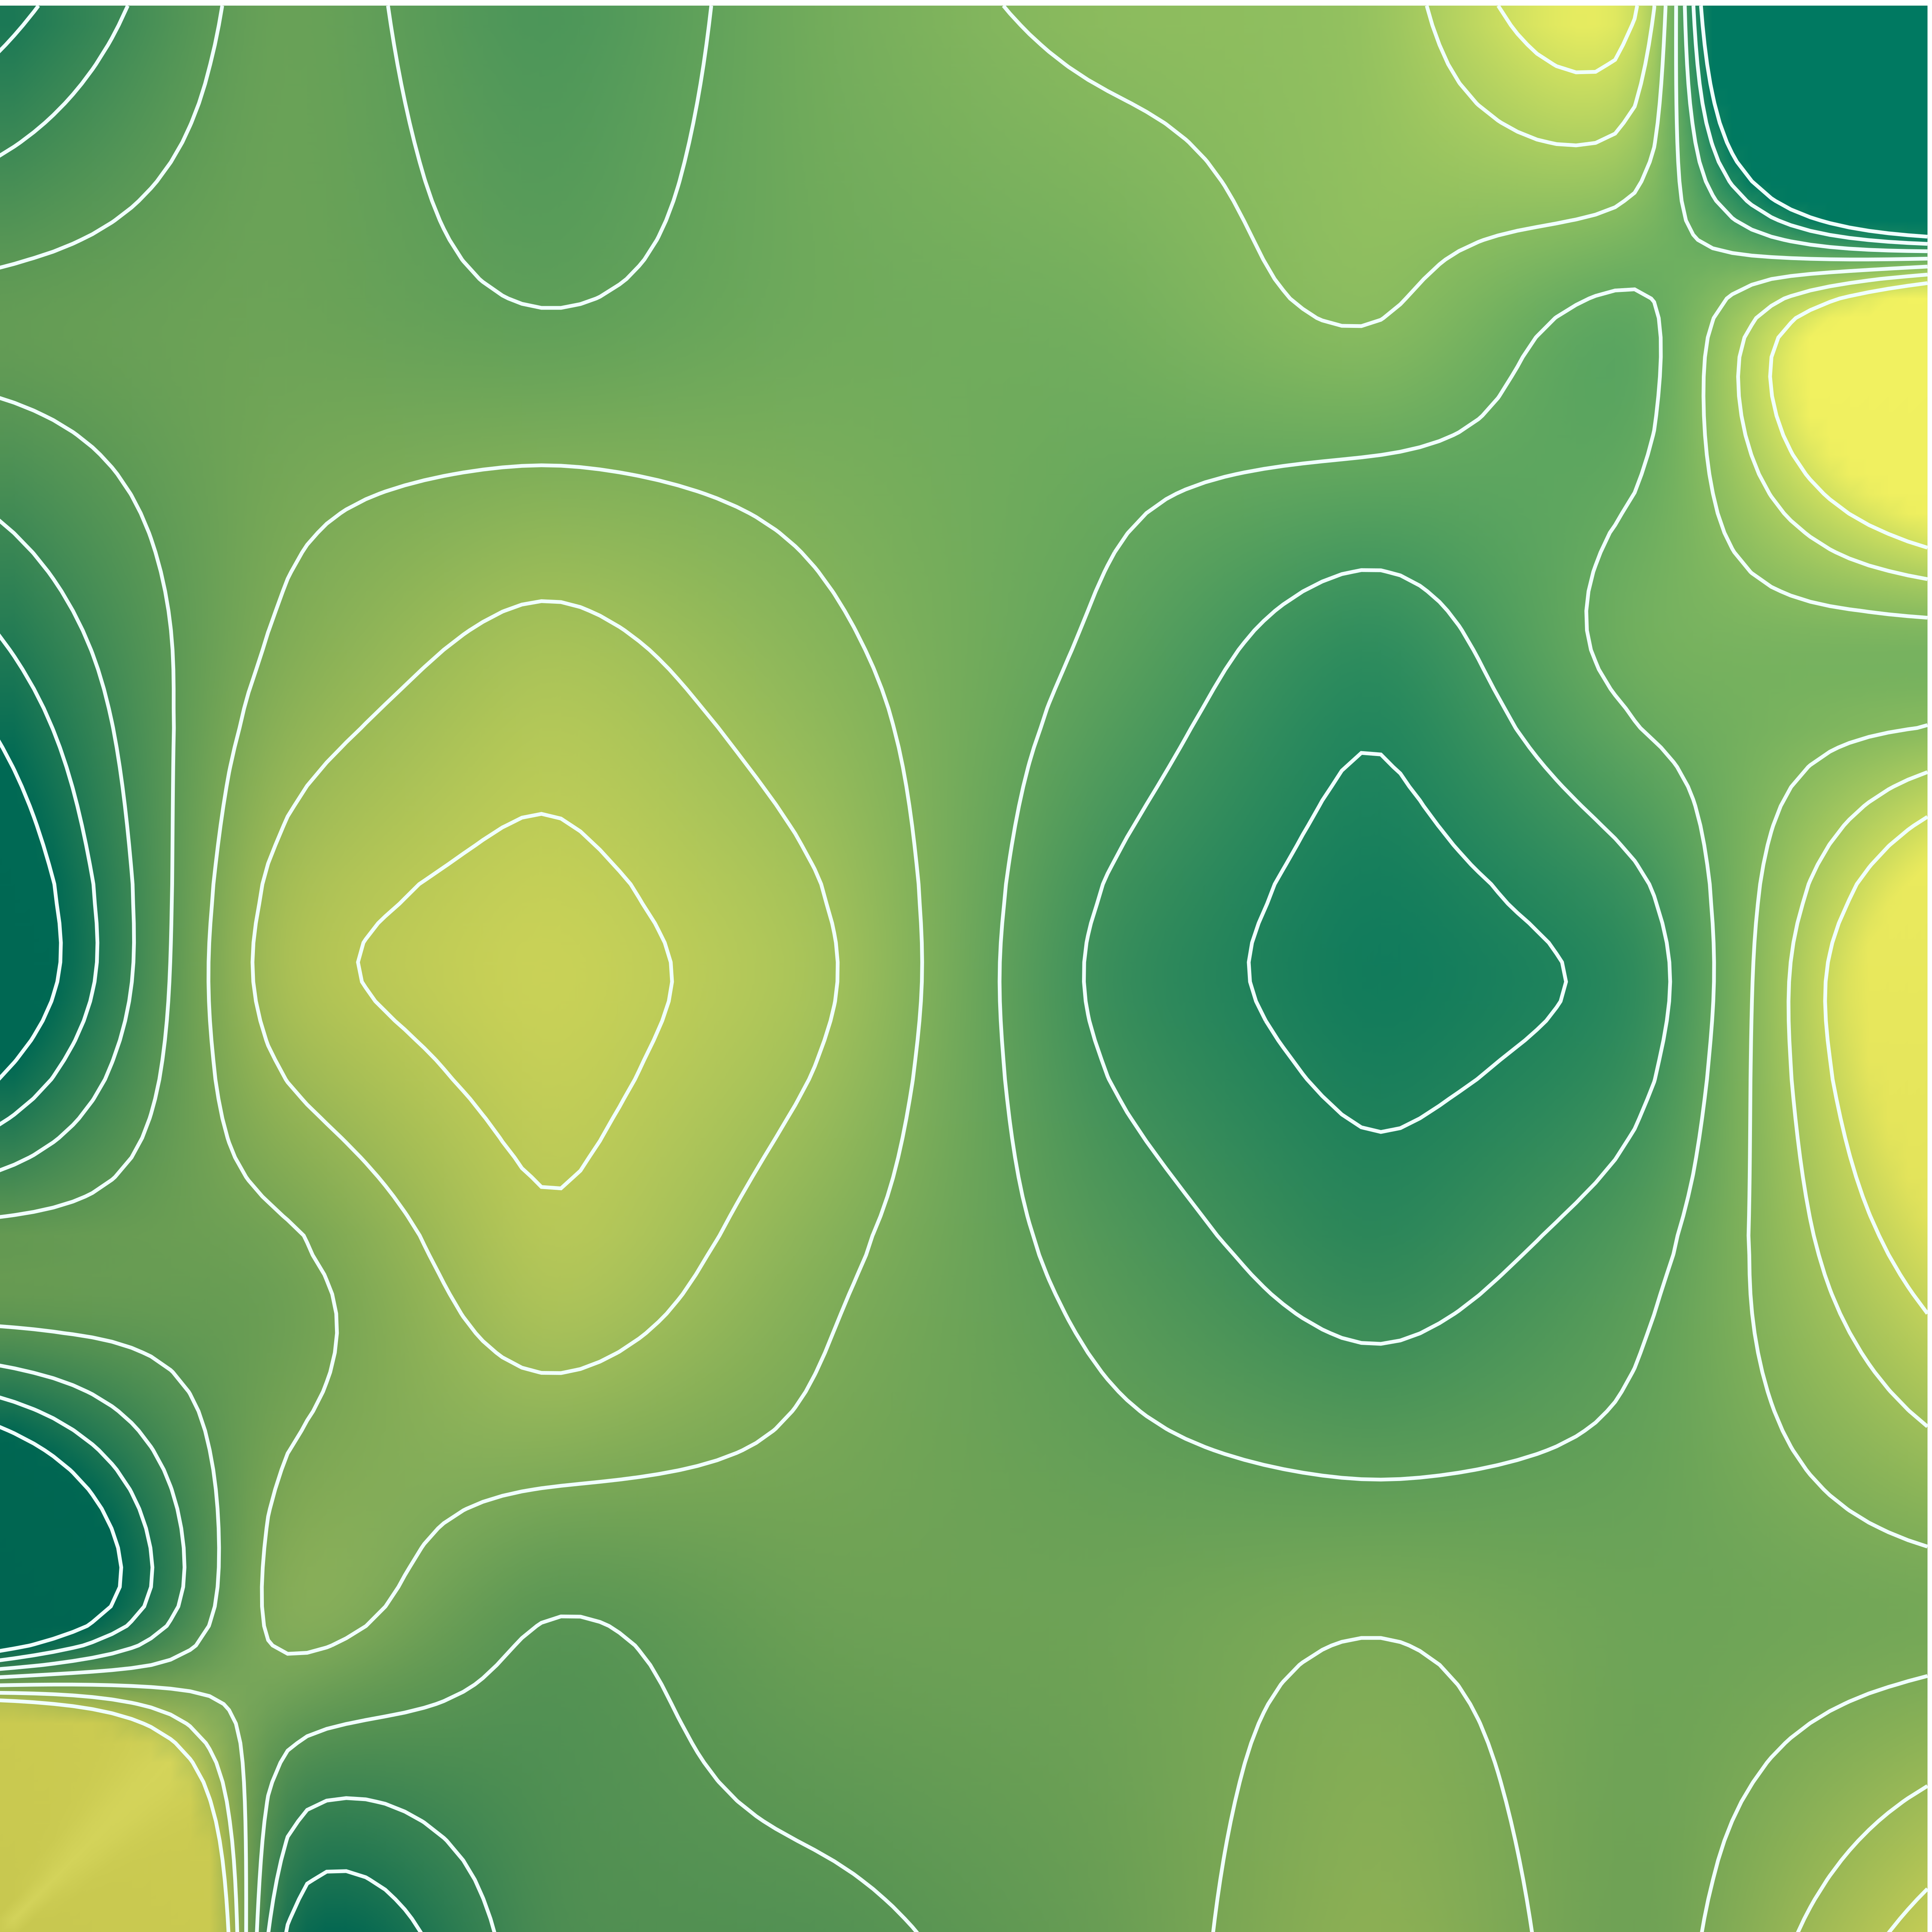
\includegraphics[width=0.4\textwidth]{figures/shearlocking/SquarePlate_T3_q1_8_7.png}}\end{subcaptiongroup}
    &\begin{subcaptiongroup}\raisebox{-0.5\height}{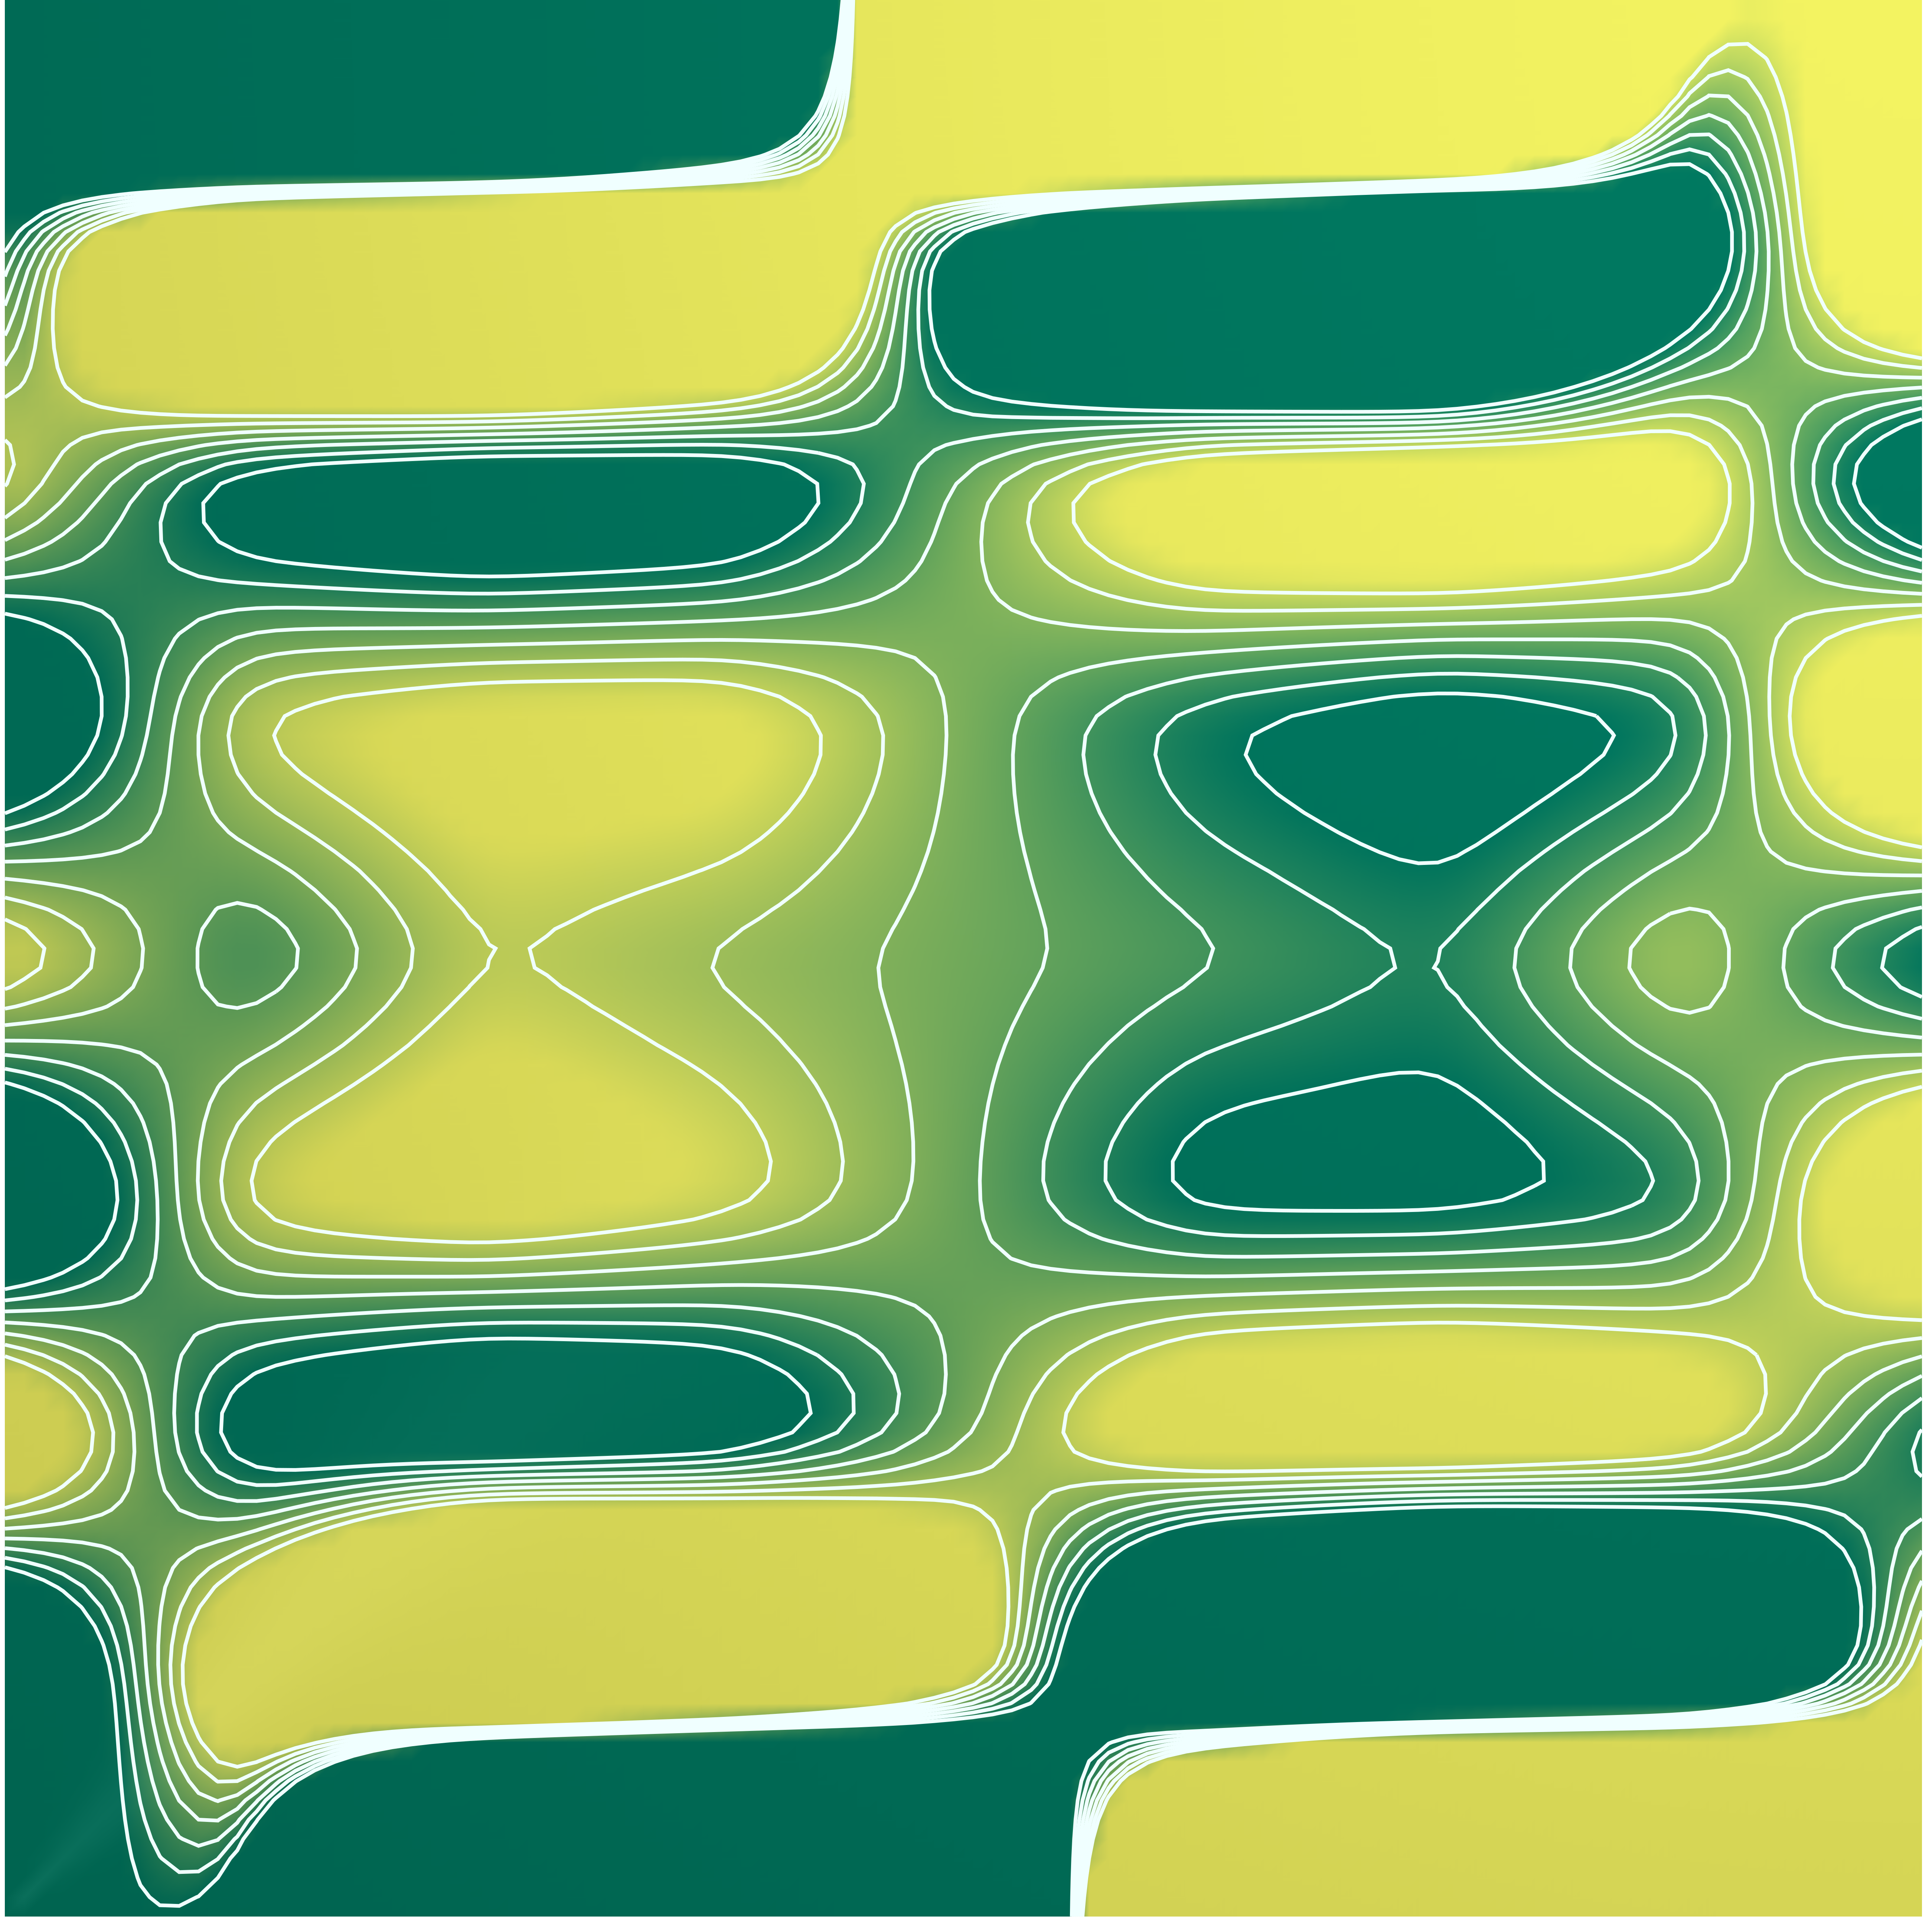
\includegraphics[width=0.4\textwidth]{figures/shearlocking/SquarePlate_T3_q1_8_8.png}}\end{subcaptiongroup}\\
    $289$&\begin{subcaptiongroup}\raisebox{-0.5\height}{\includegraphics[width=0.4\textwidth]{figures/shearlocking/SquarePlate_T3_q1_16_13.png}}\end{subcaptiongroup}
    &\begin{subcaptiongroup}\raisebox{-0.5\height}{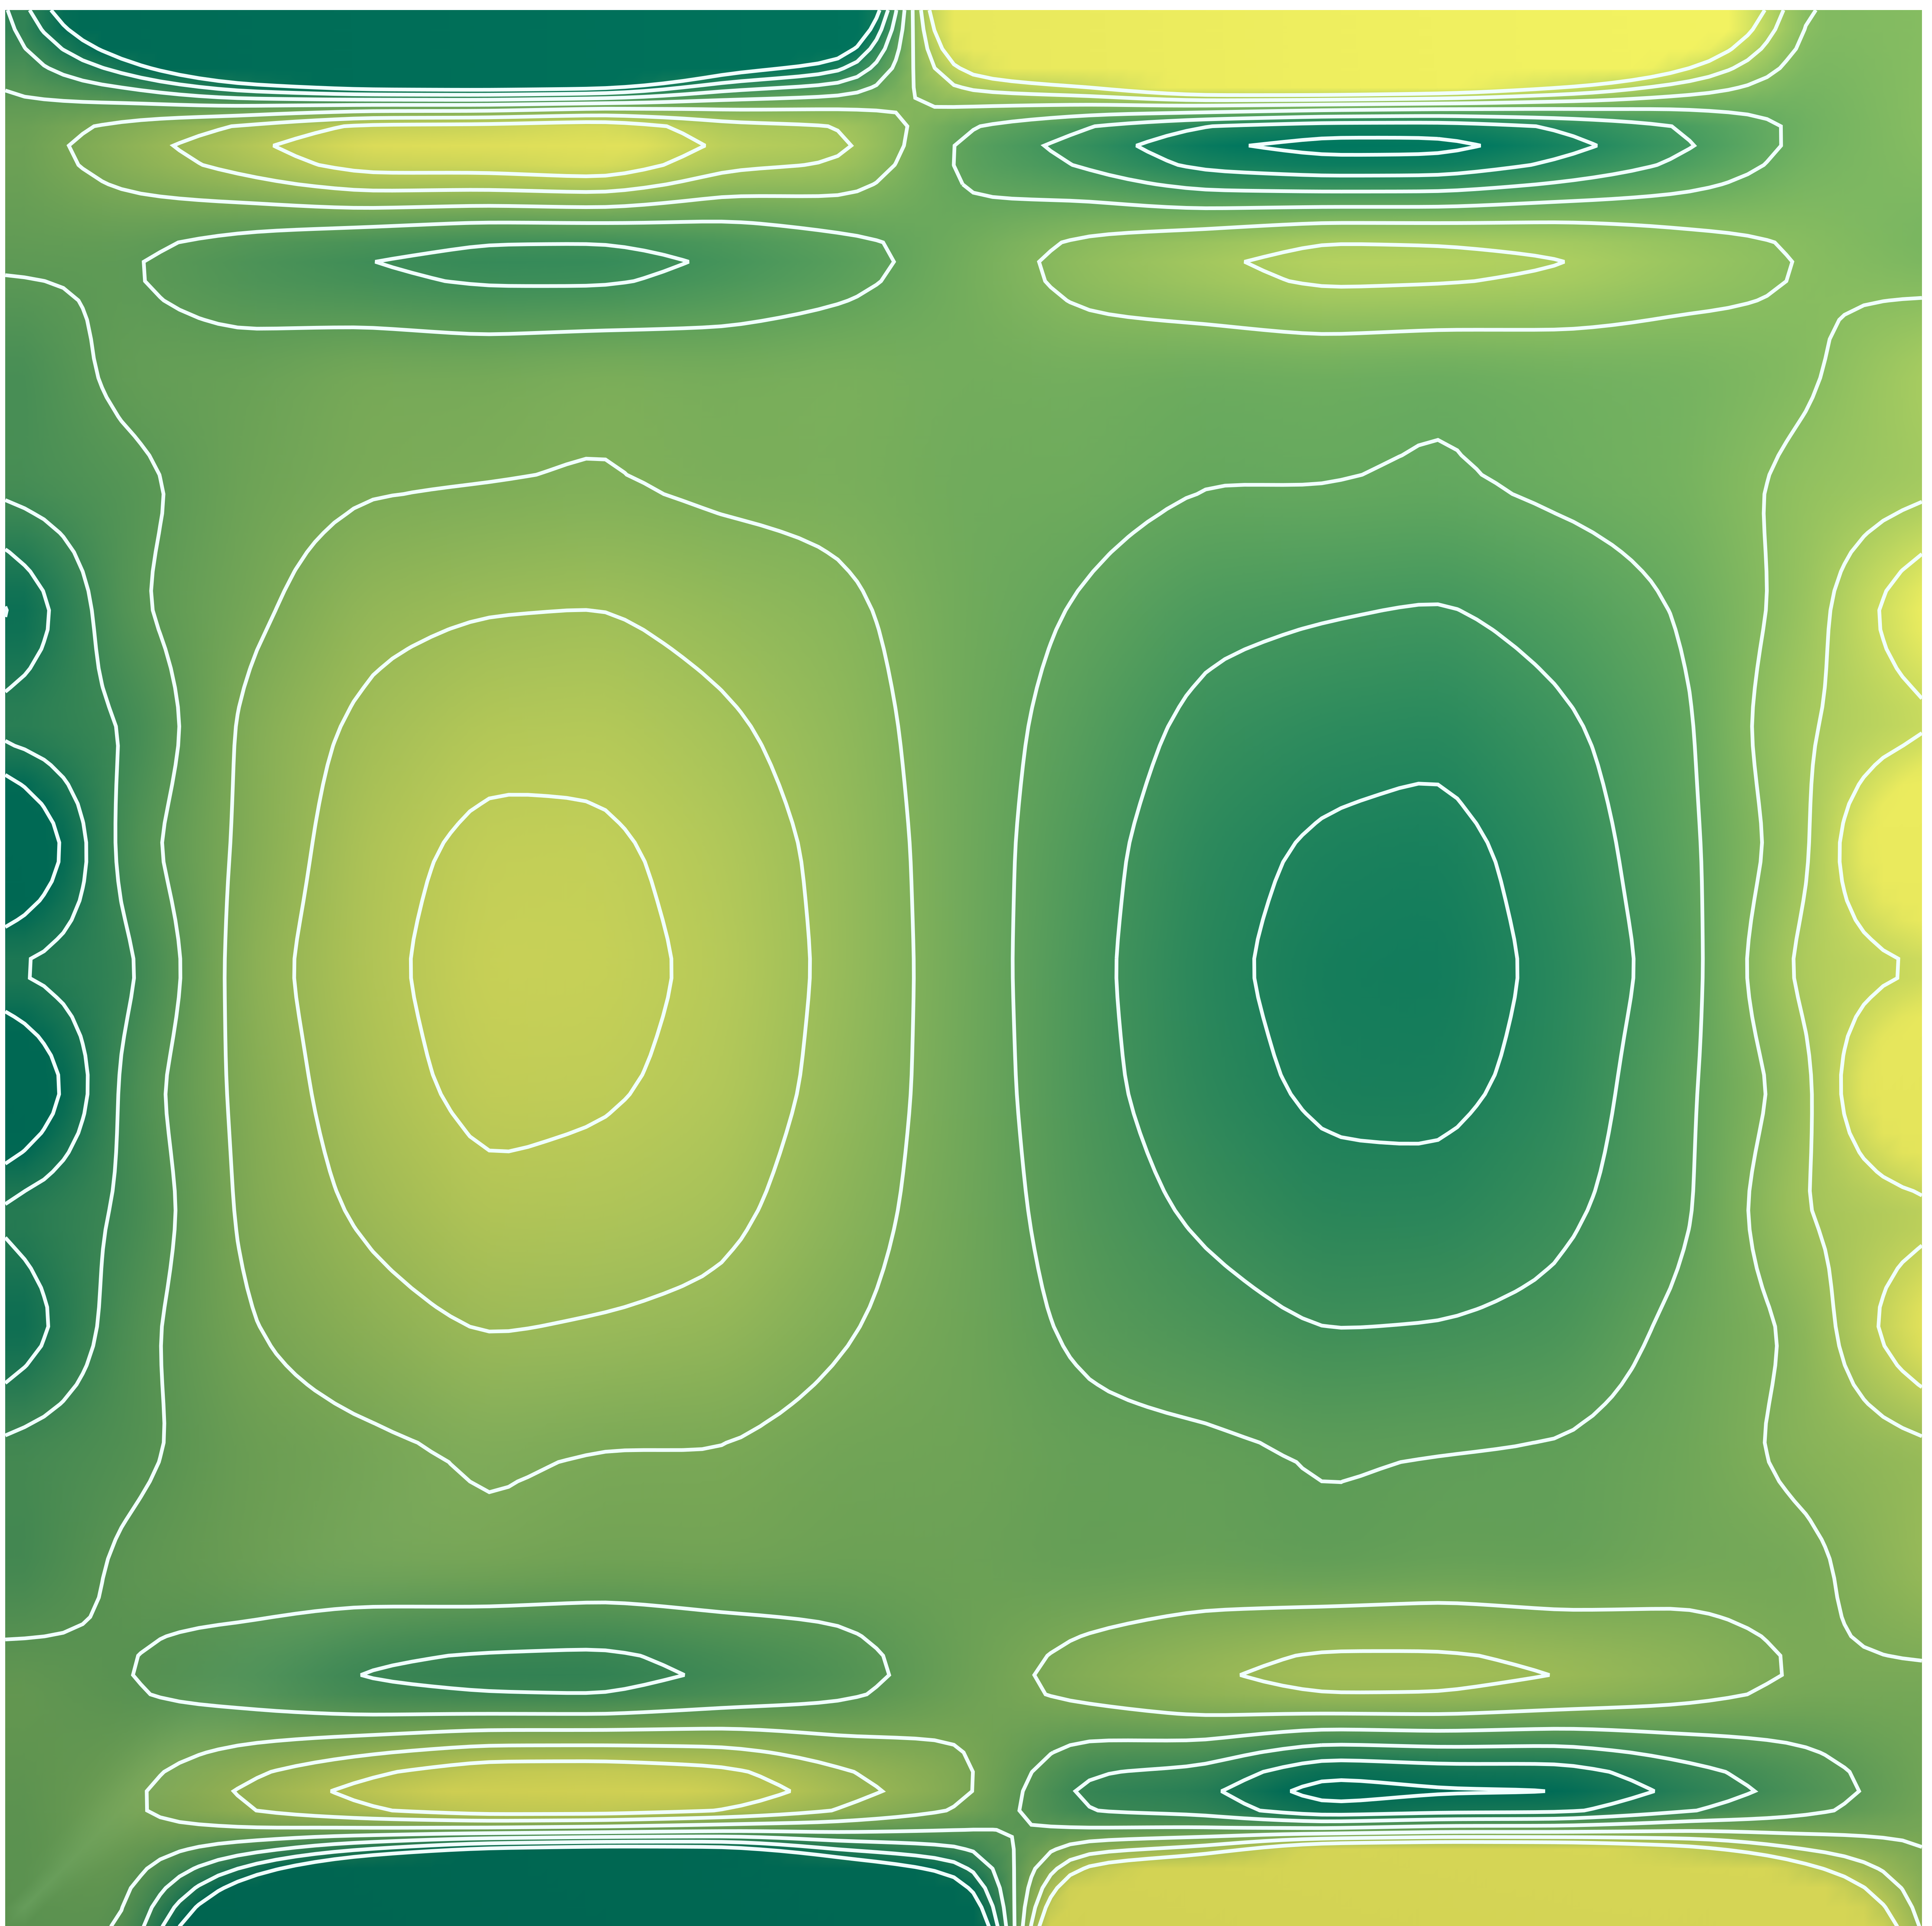
\includegraphics[width=0.4\textwidth]{figures/shearlocking/SquarePlate_T3_q1_16_16.png}}\end{subcaptiongroup}\\
    $1089$&\begin{subcaptiongroup}\raisebox{-0.5\height}{\includegraphics[width=0.4\textwidth]{figures/shearlocking/SquarePlate_T3_q1_32_26.png}}\end{subcaptiongroup}
    &\begin{subcaptiongroup}\raisebox{-0.5\height}{\includegraphics[width=0.4\textwidth]{figures/shearlocking/SquarePlate_T3_q1_32_32.png}}\end{subcaptiongroup}\\
    \end{tabular}
    \caption{\textbf{固支方板问题Tri3单元应力云图($Q_1$)}}\label{Q1-Tri3}
\end{figure}

\begin{figure}[H]
    \centering
    \begin{tabular}{cccc}
    $\quad$&最优约束比&传统约束比\\
    $81$&\begin{subcaptiongroup}\raisebox{-0.5\height}{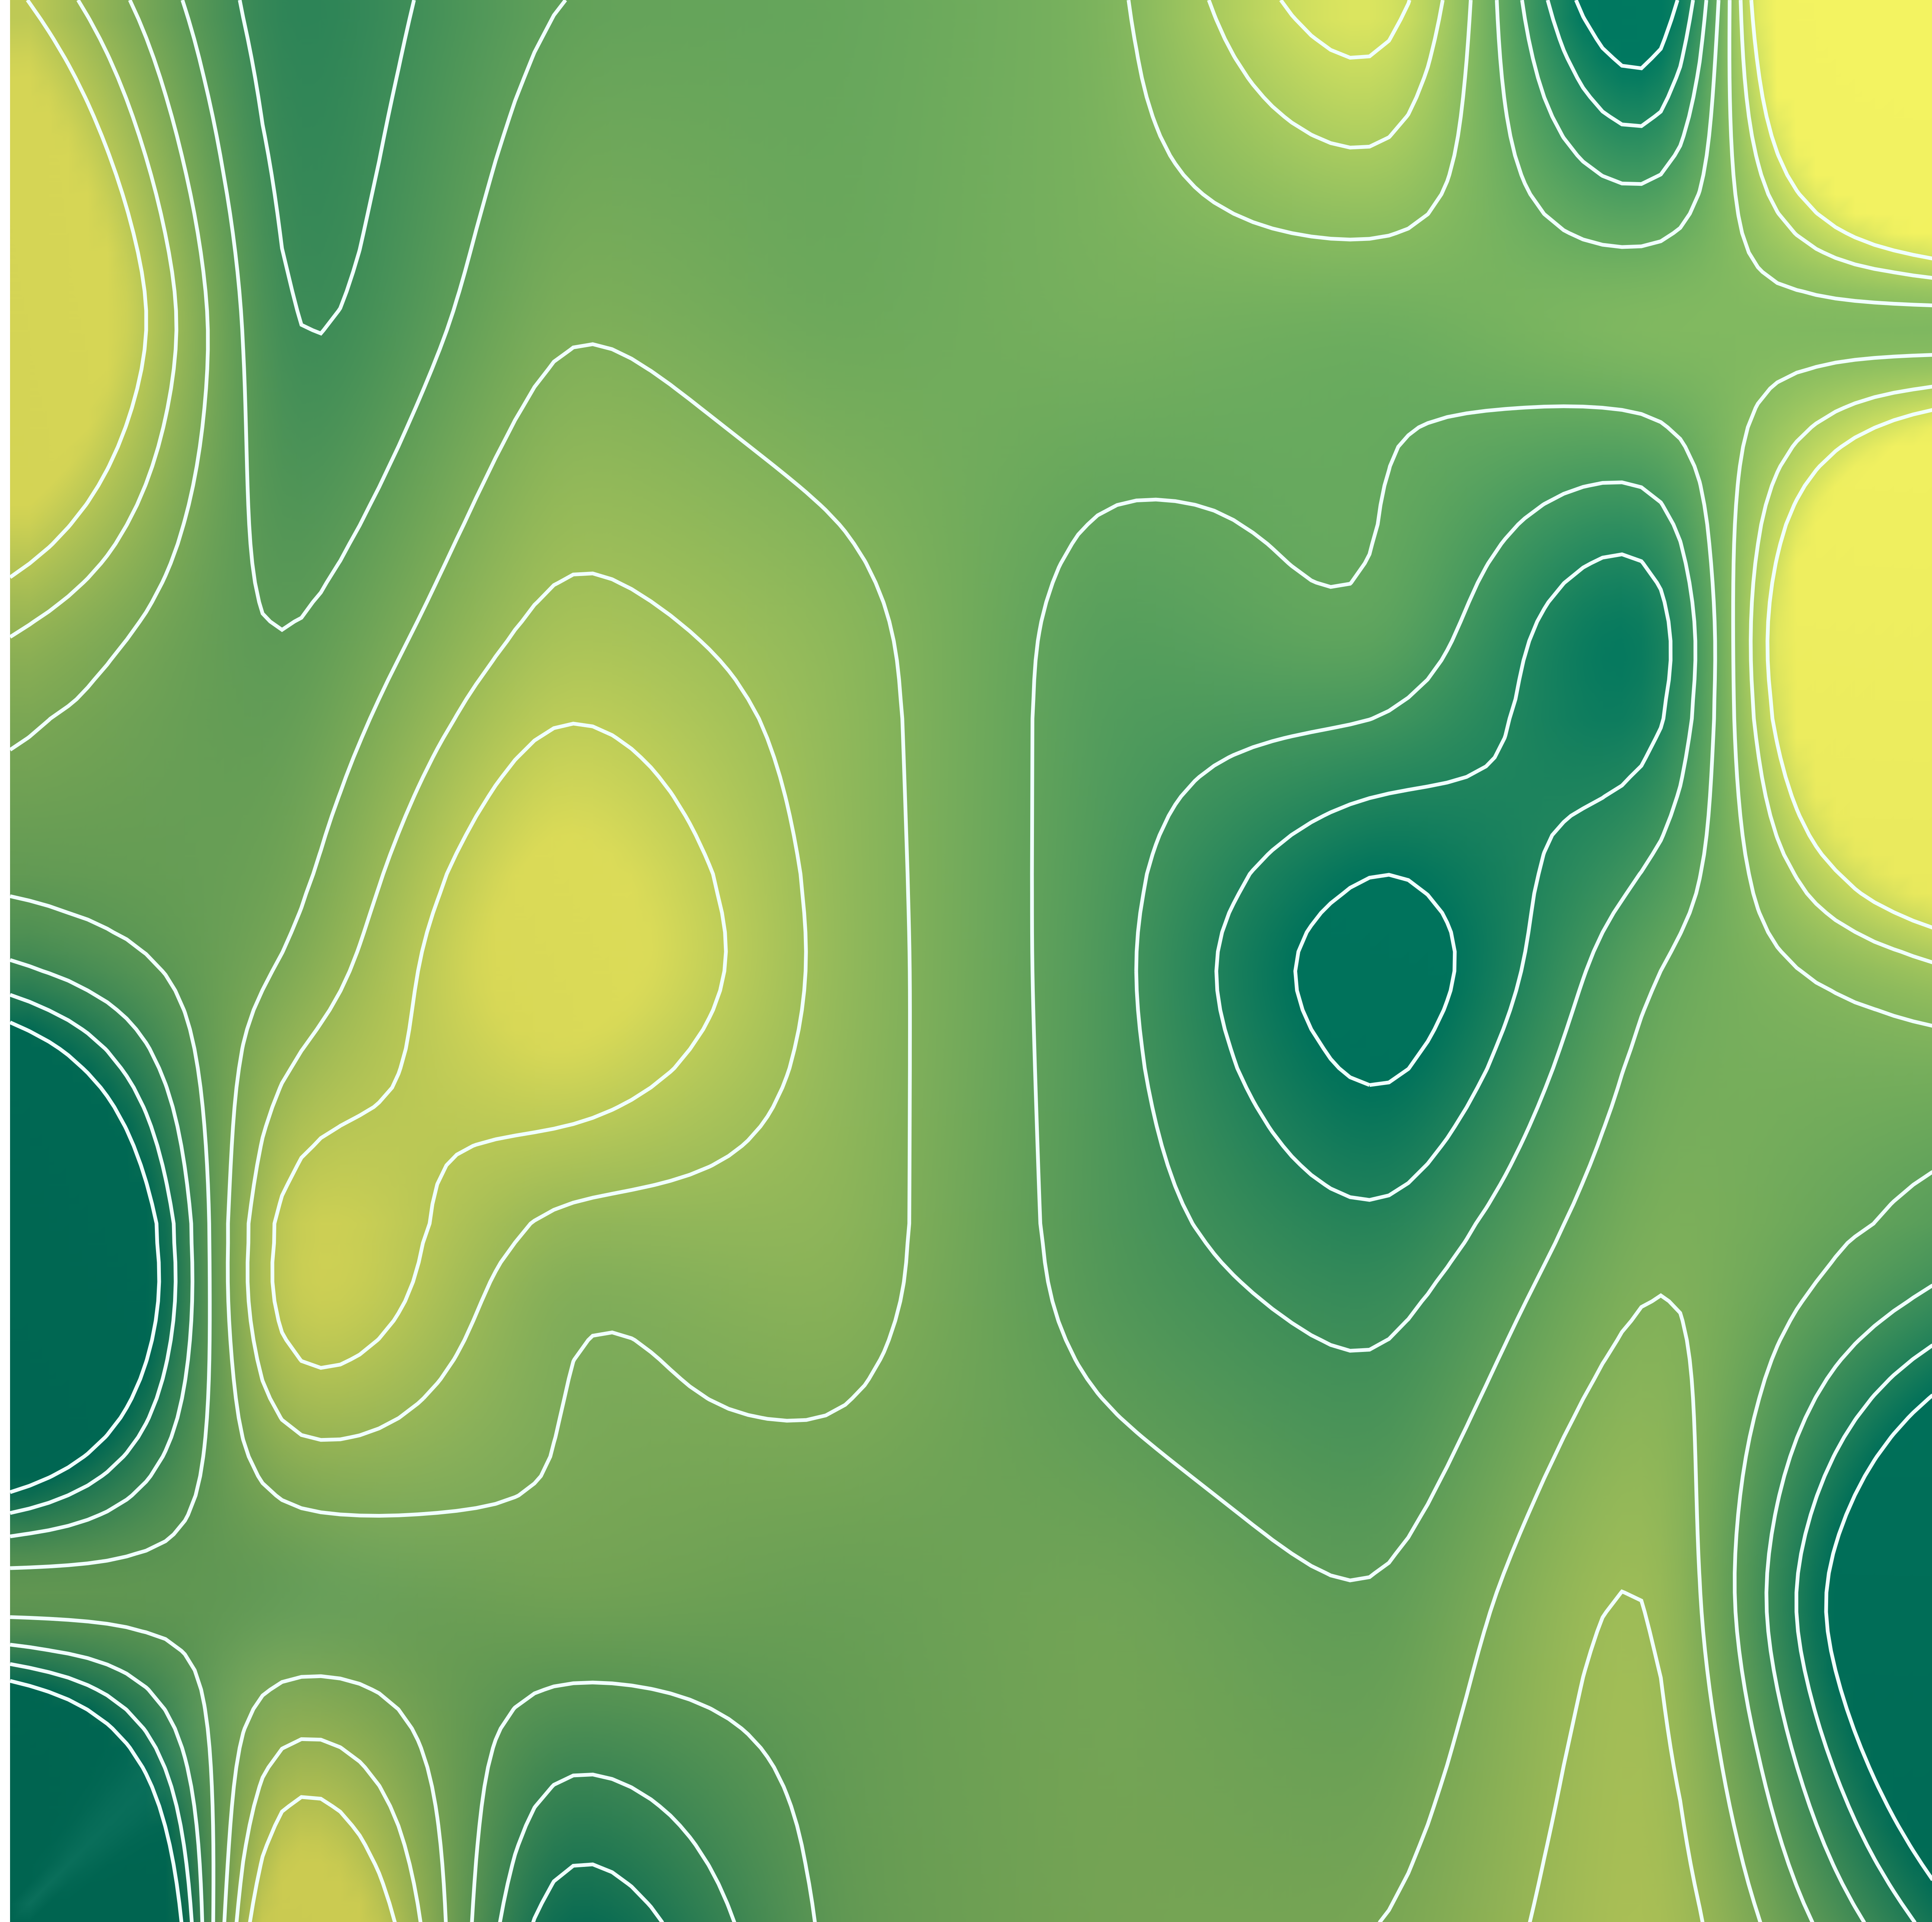
\includegraphics[width=0.4\textwidth]{figures/shearlocking/SquarePlate_mix_quad4_q1_8_7.png}}\end{subcaptiongroup}
    &\begin{subcaptiongroup}\raisebox{-0.5\height}{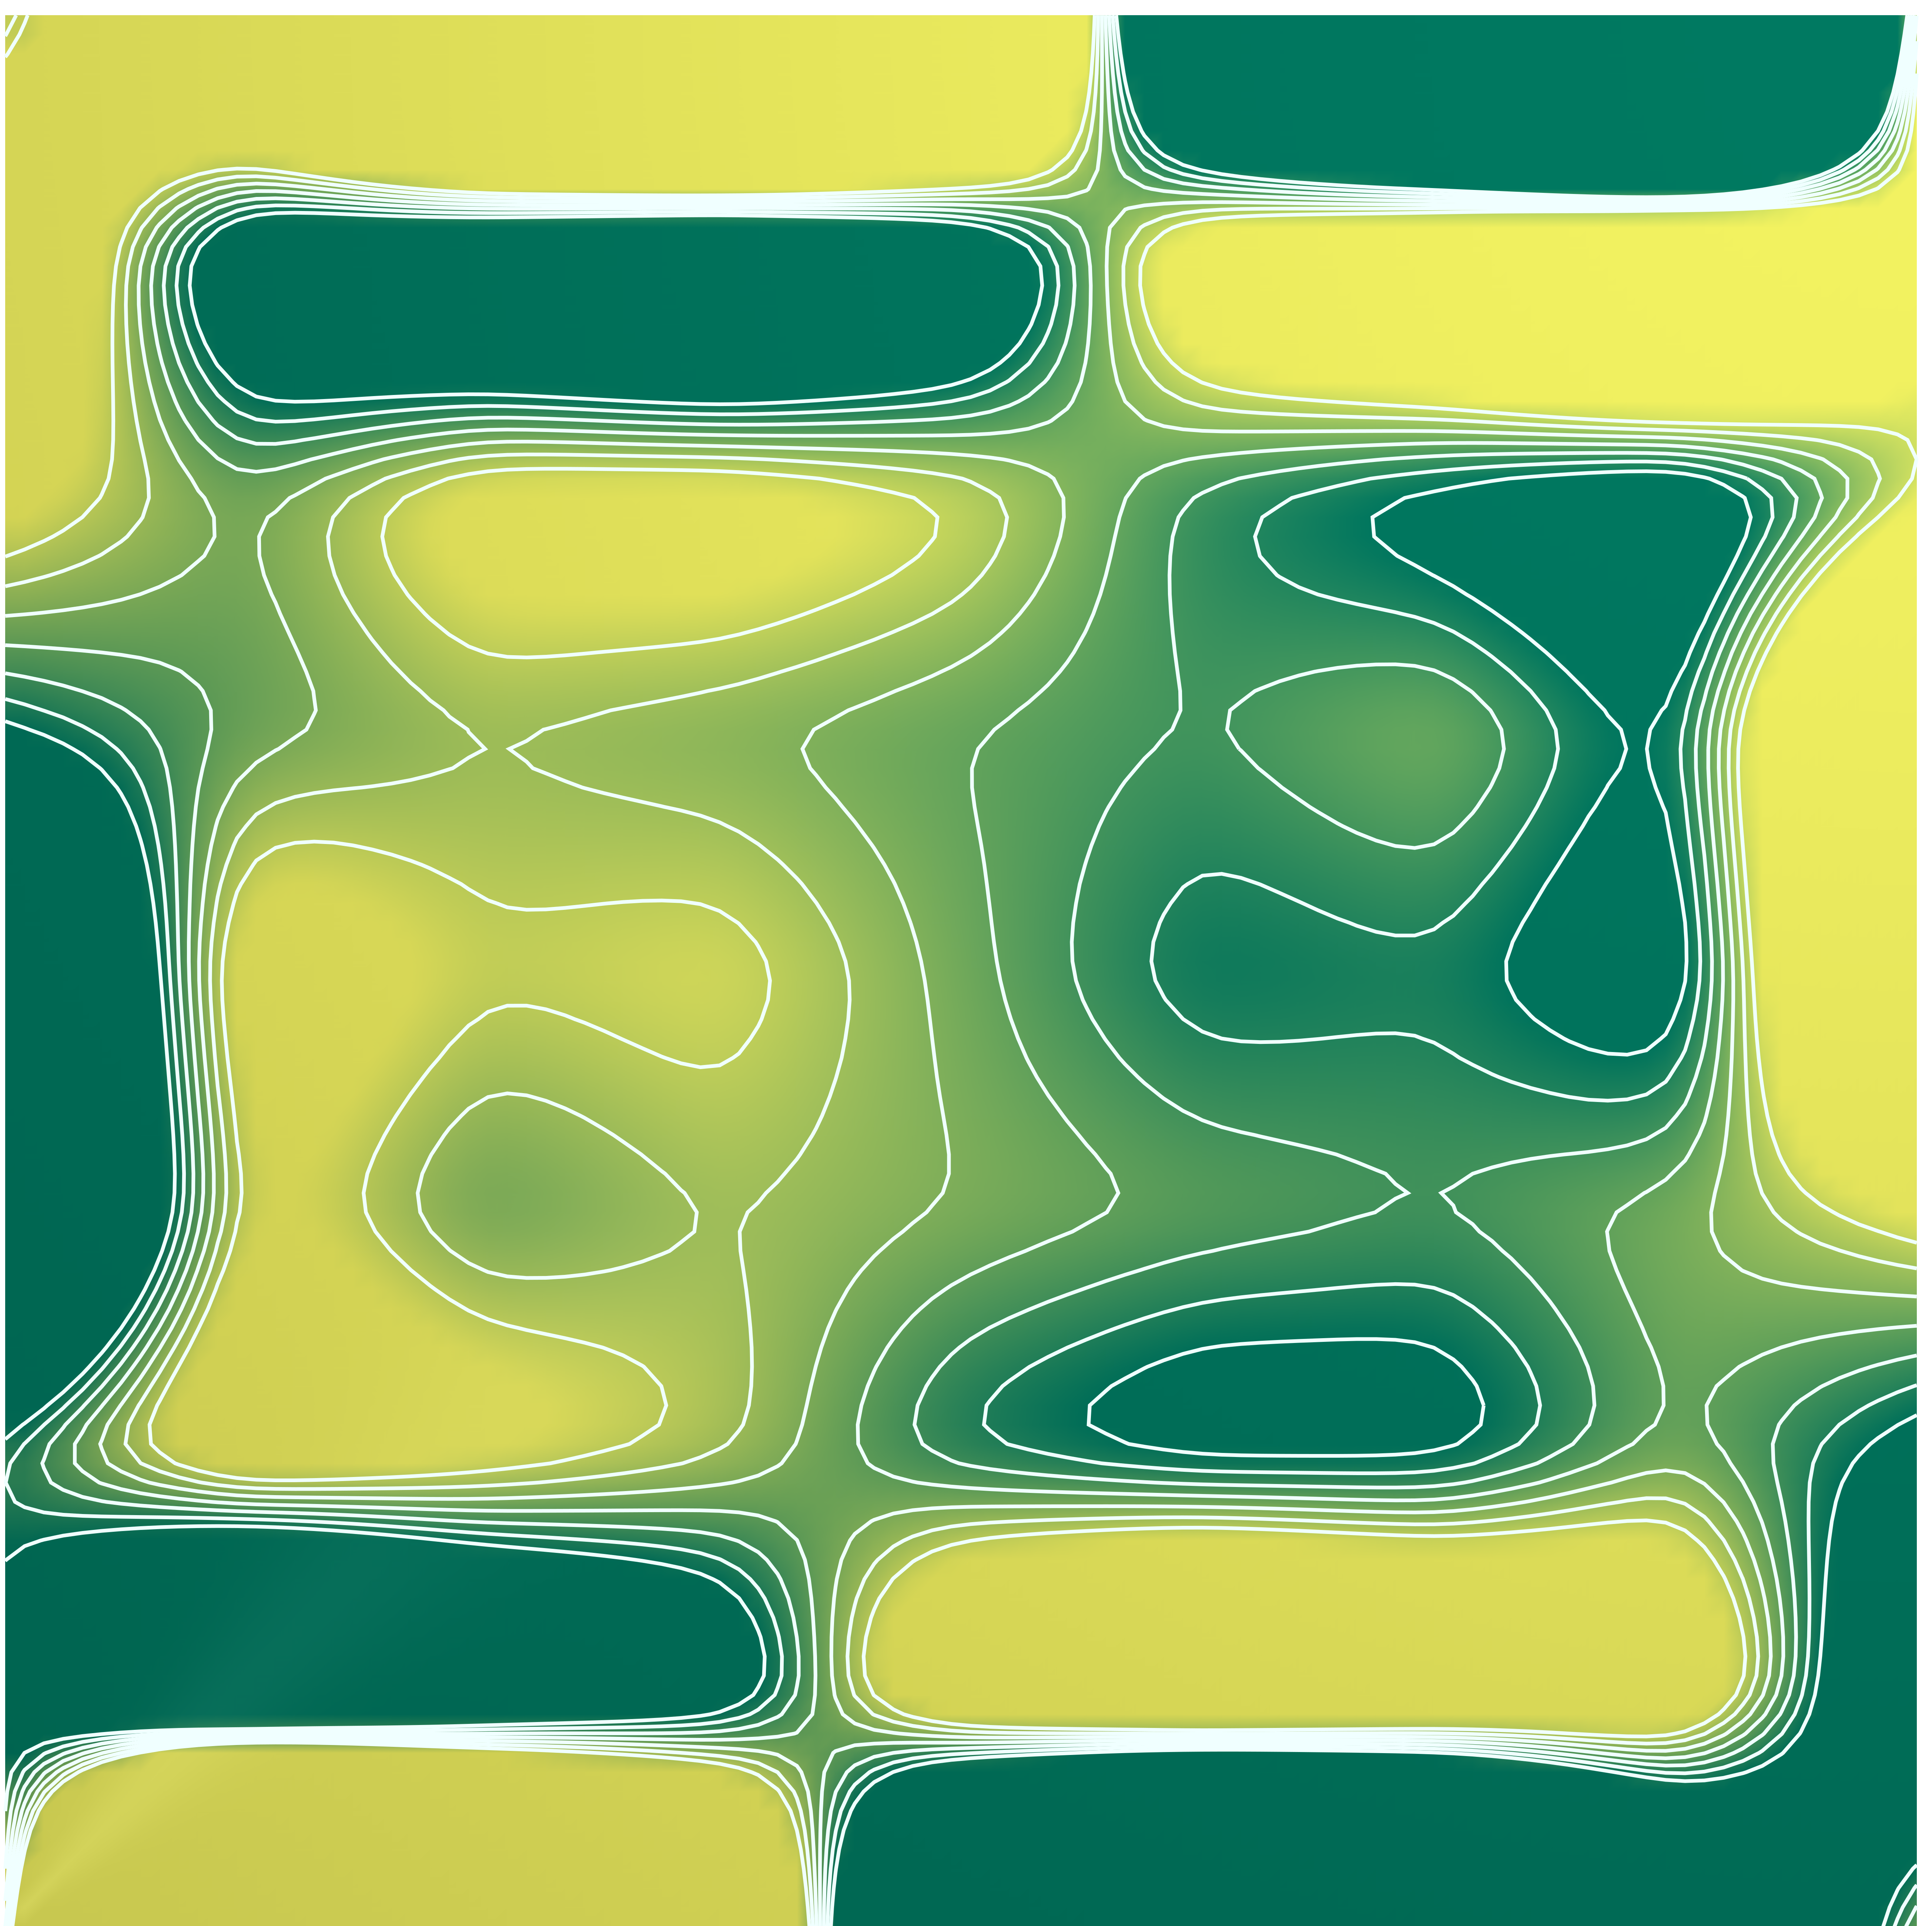
\includegraphics[width=0.4\textwidth]{figures/shearlocking/SquarePlate_mix_quad4_q1_8_8.png}}\end{subcaptiongroup}\\
    $289$&\begin{subcaptiongroup}\raisebox{-0.5\height}{\includegraphics[width=0.4\textwidth]{figures/shearlocking/SquarePlate_mix_quad4_q1_16_13.png}}\end{subcaptiongroup}
    &\begin{subcaptiongroup}\raisebox{-0.5\height}{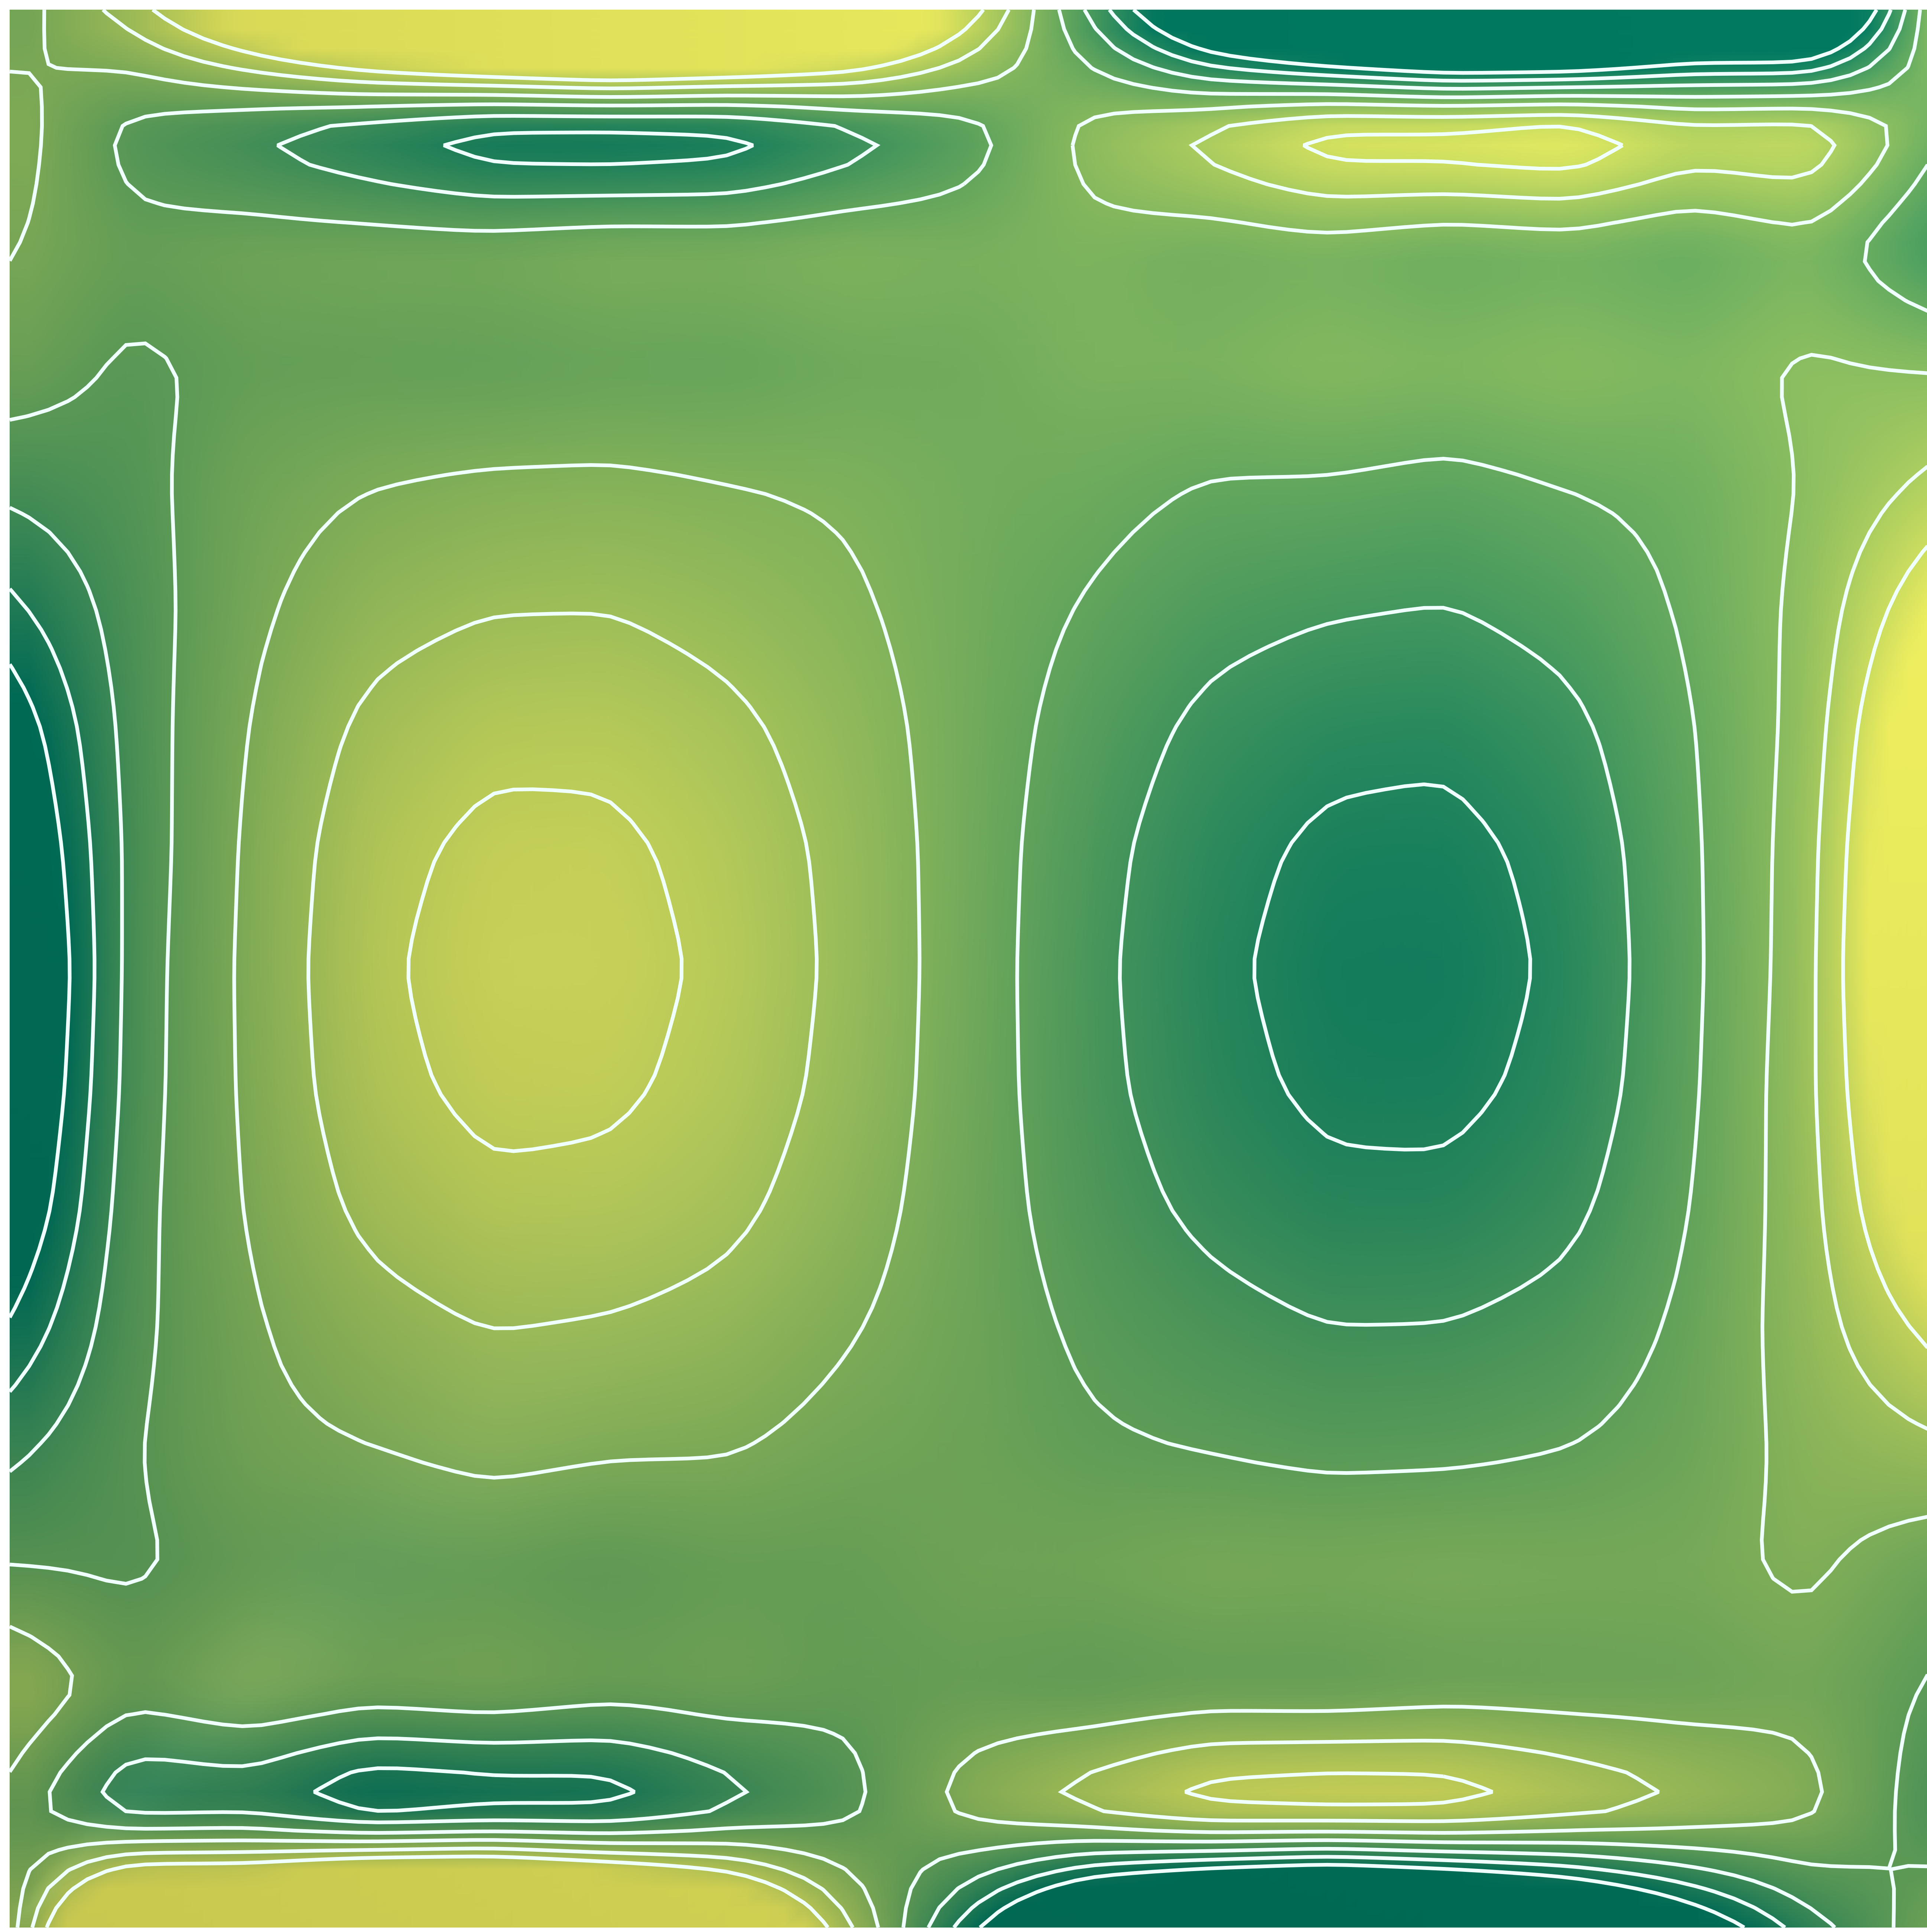
\includegraphics[width=0.4\textwidth]{figures/shearlocking/SquarePlate_mix_quad4_q1_16_16.png}}\end{subcaptiongroup}\\
    $1089$&\begin{subcaptiongroup}\raisebox{-0.5\height}{\includegraphics[width=0.4\textwidth]{figures/shearlocking/SquarePlate_mix_quad4_q1_32_26.png}}\end{subcaptiongroup}
    &\begin{subcaptiongroup}\raisebox{-0.5\height}{\includegraphics[width=0.4\textwidth]{figures/shearlocking/SquarePlate_mix_quad4_q1_32_32.png}}\end{subcaptiongroup}\\
    \end{tabular}
    \caption{\textbf{固支方板问题Quad4单元应力云图($Q_1$)}}\label{Q1-Quad4}
\end{figure}

\begin{figure}[H]
    \centering
    \begin{tabular}{cccc}
    $\quad$&最优约束比&传统约束比\\
    $289$&\begin{subcaptiongroup}\raisebox{-0.5\height}{\includegraphics[width=0.4\textwidth]{figures/shearlocking/SquarePlate_mix_tri6_q1_8_6.png}}\end{subcaptiongroup}
    &\begin{subcaptiongroup}\raisebox{-0.5\height}{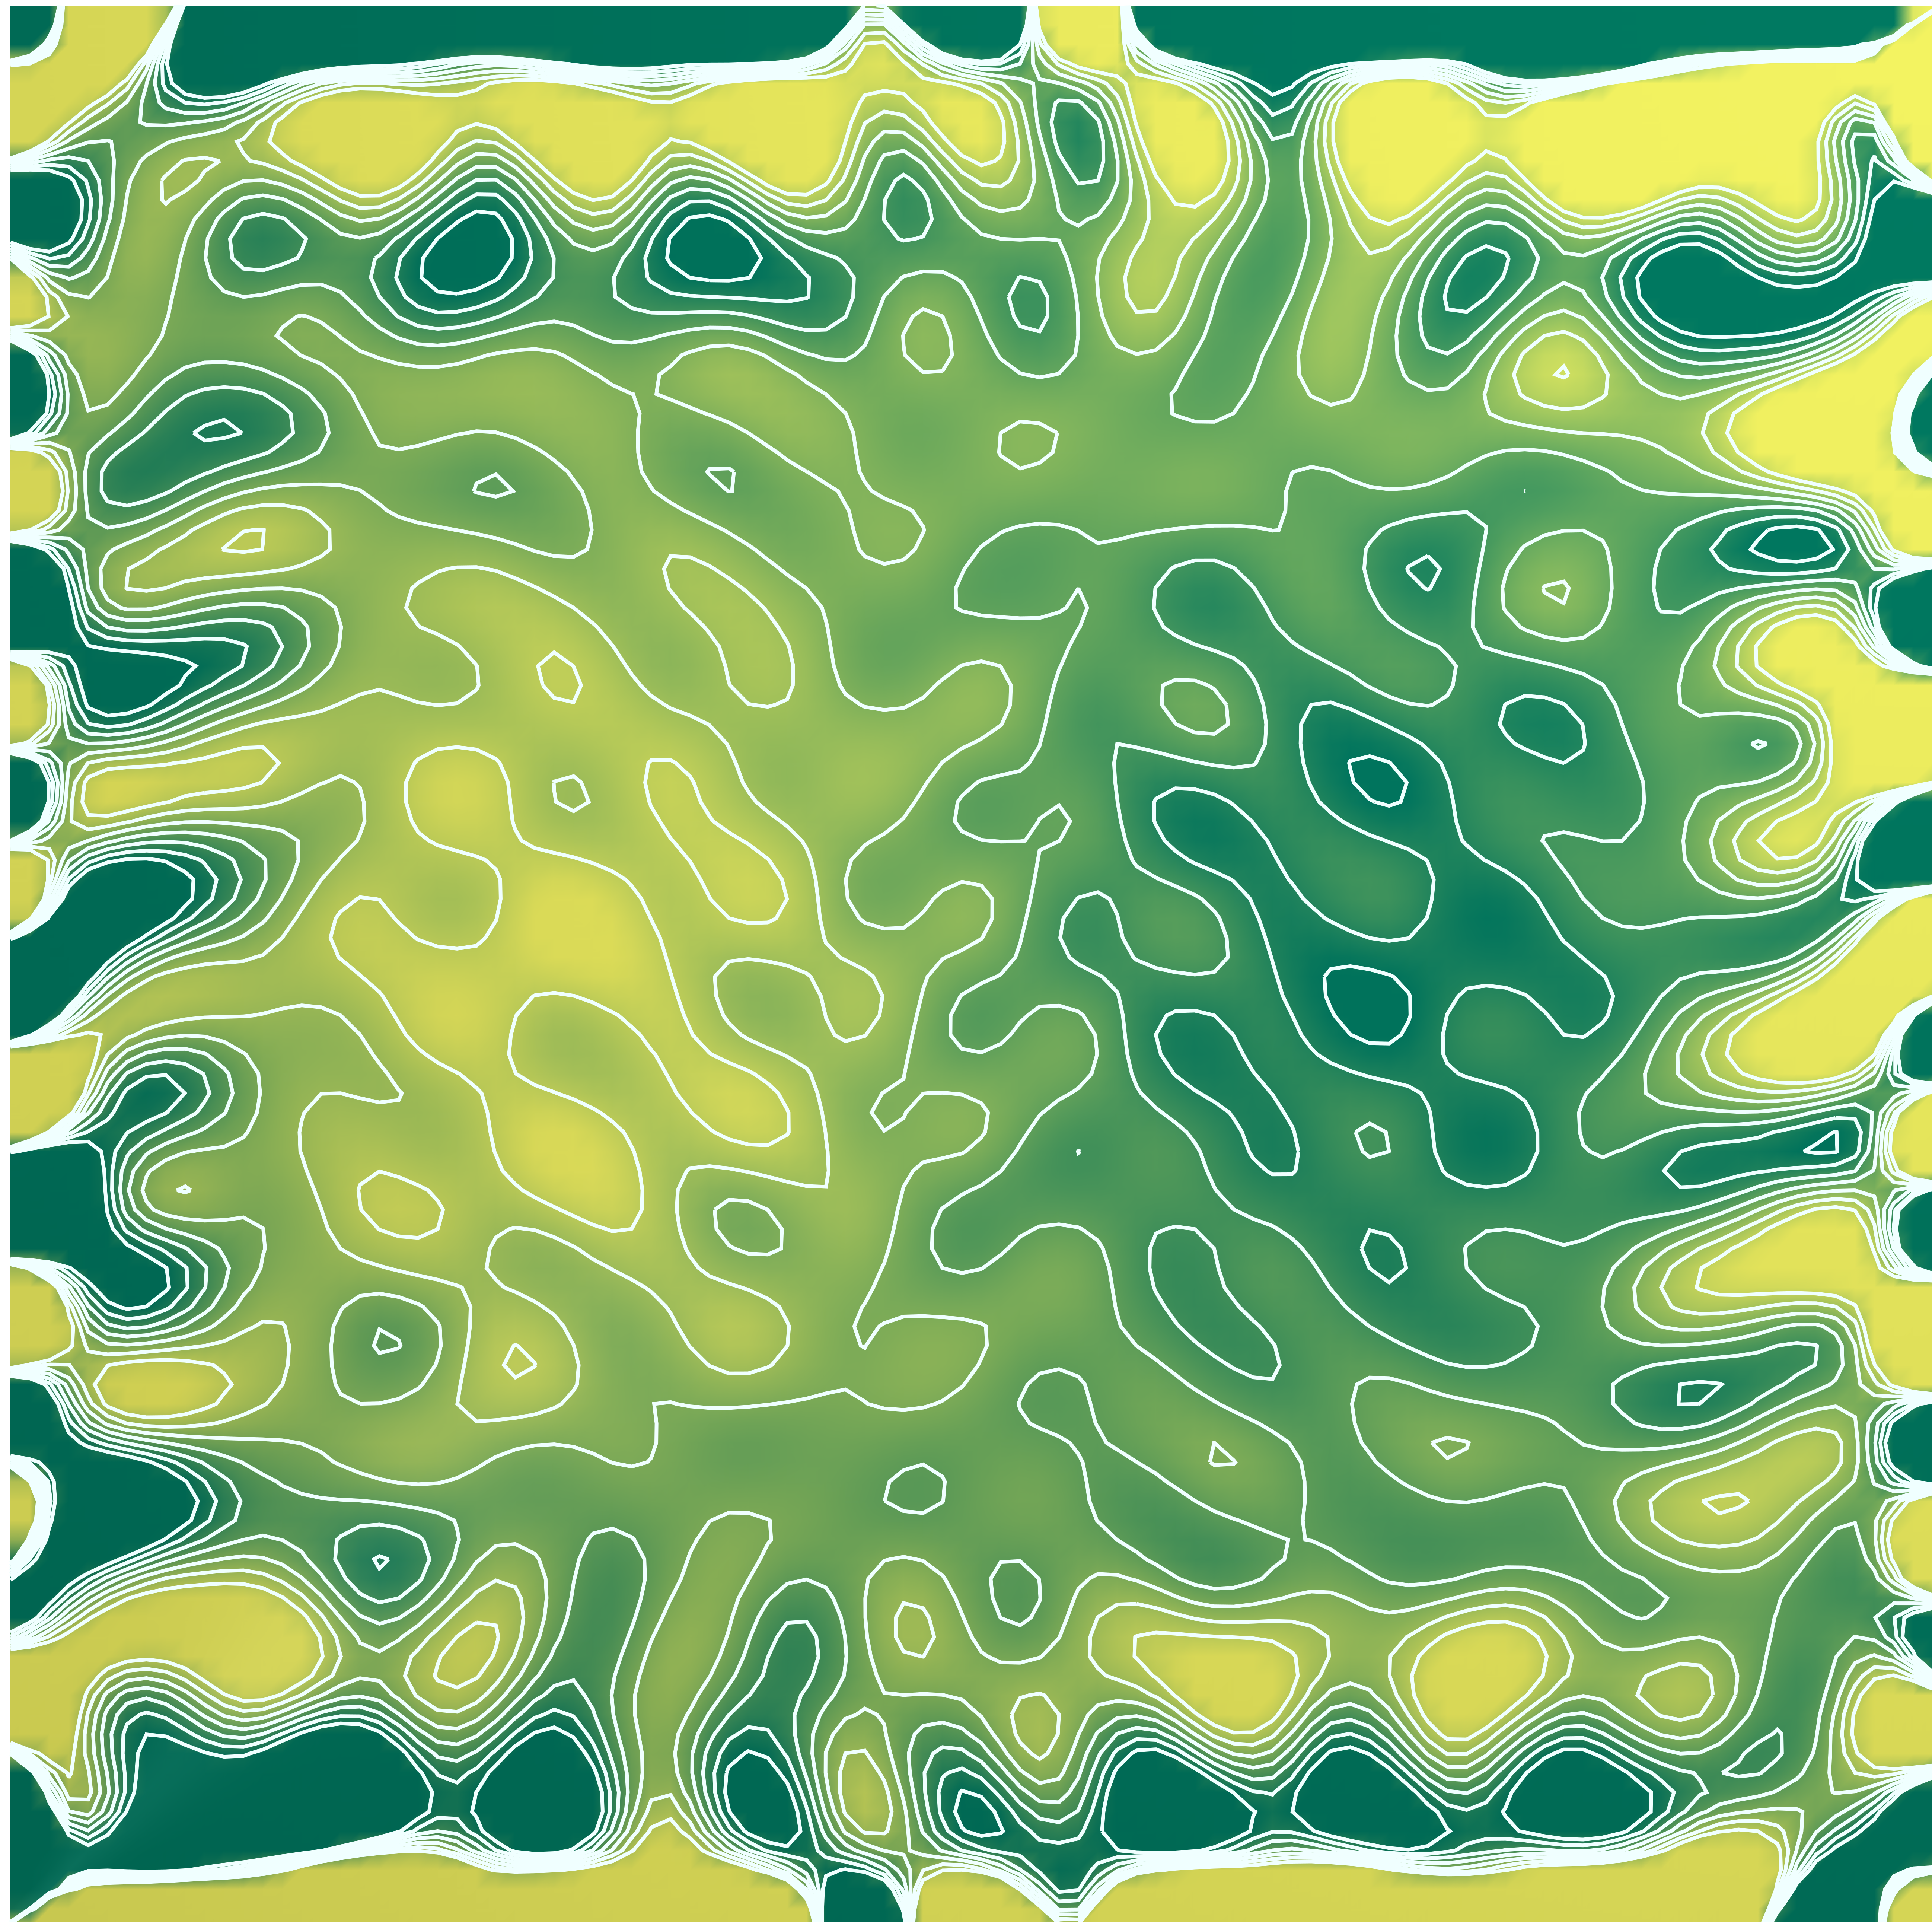
\includegraphics[width=0.4\textwidth]{figures/shearlocking/SquarePlate_mix_tri6_q1_8_8.png}}\end{subcaptiongroup}\\
    $1089$&\begin{subcaptiongroup}\raisebox{-0.5\height}{\includegraphics[width=0.4\textwidth]{figures/shearlocking/SquarePlate_mix_tri6_q1_16_12.png}}\end{subcaptiongroup}
    &\begin{subcaptiongroup}\raisebox{-0.5\height}{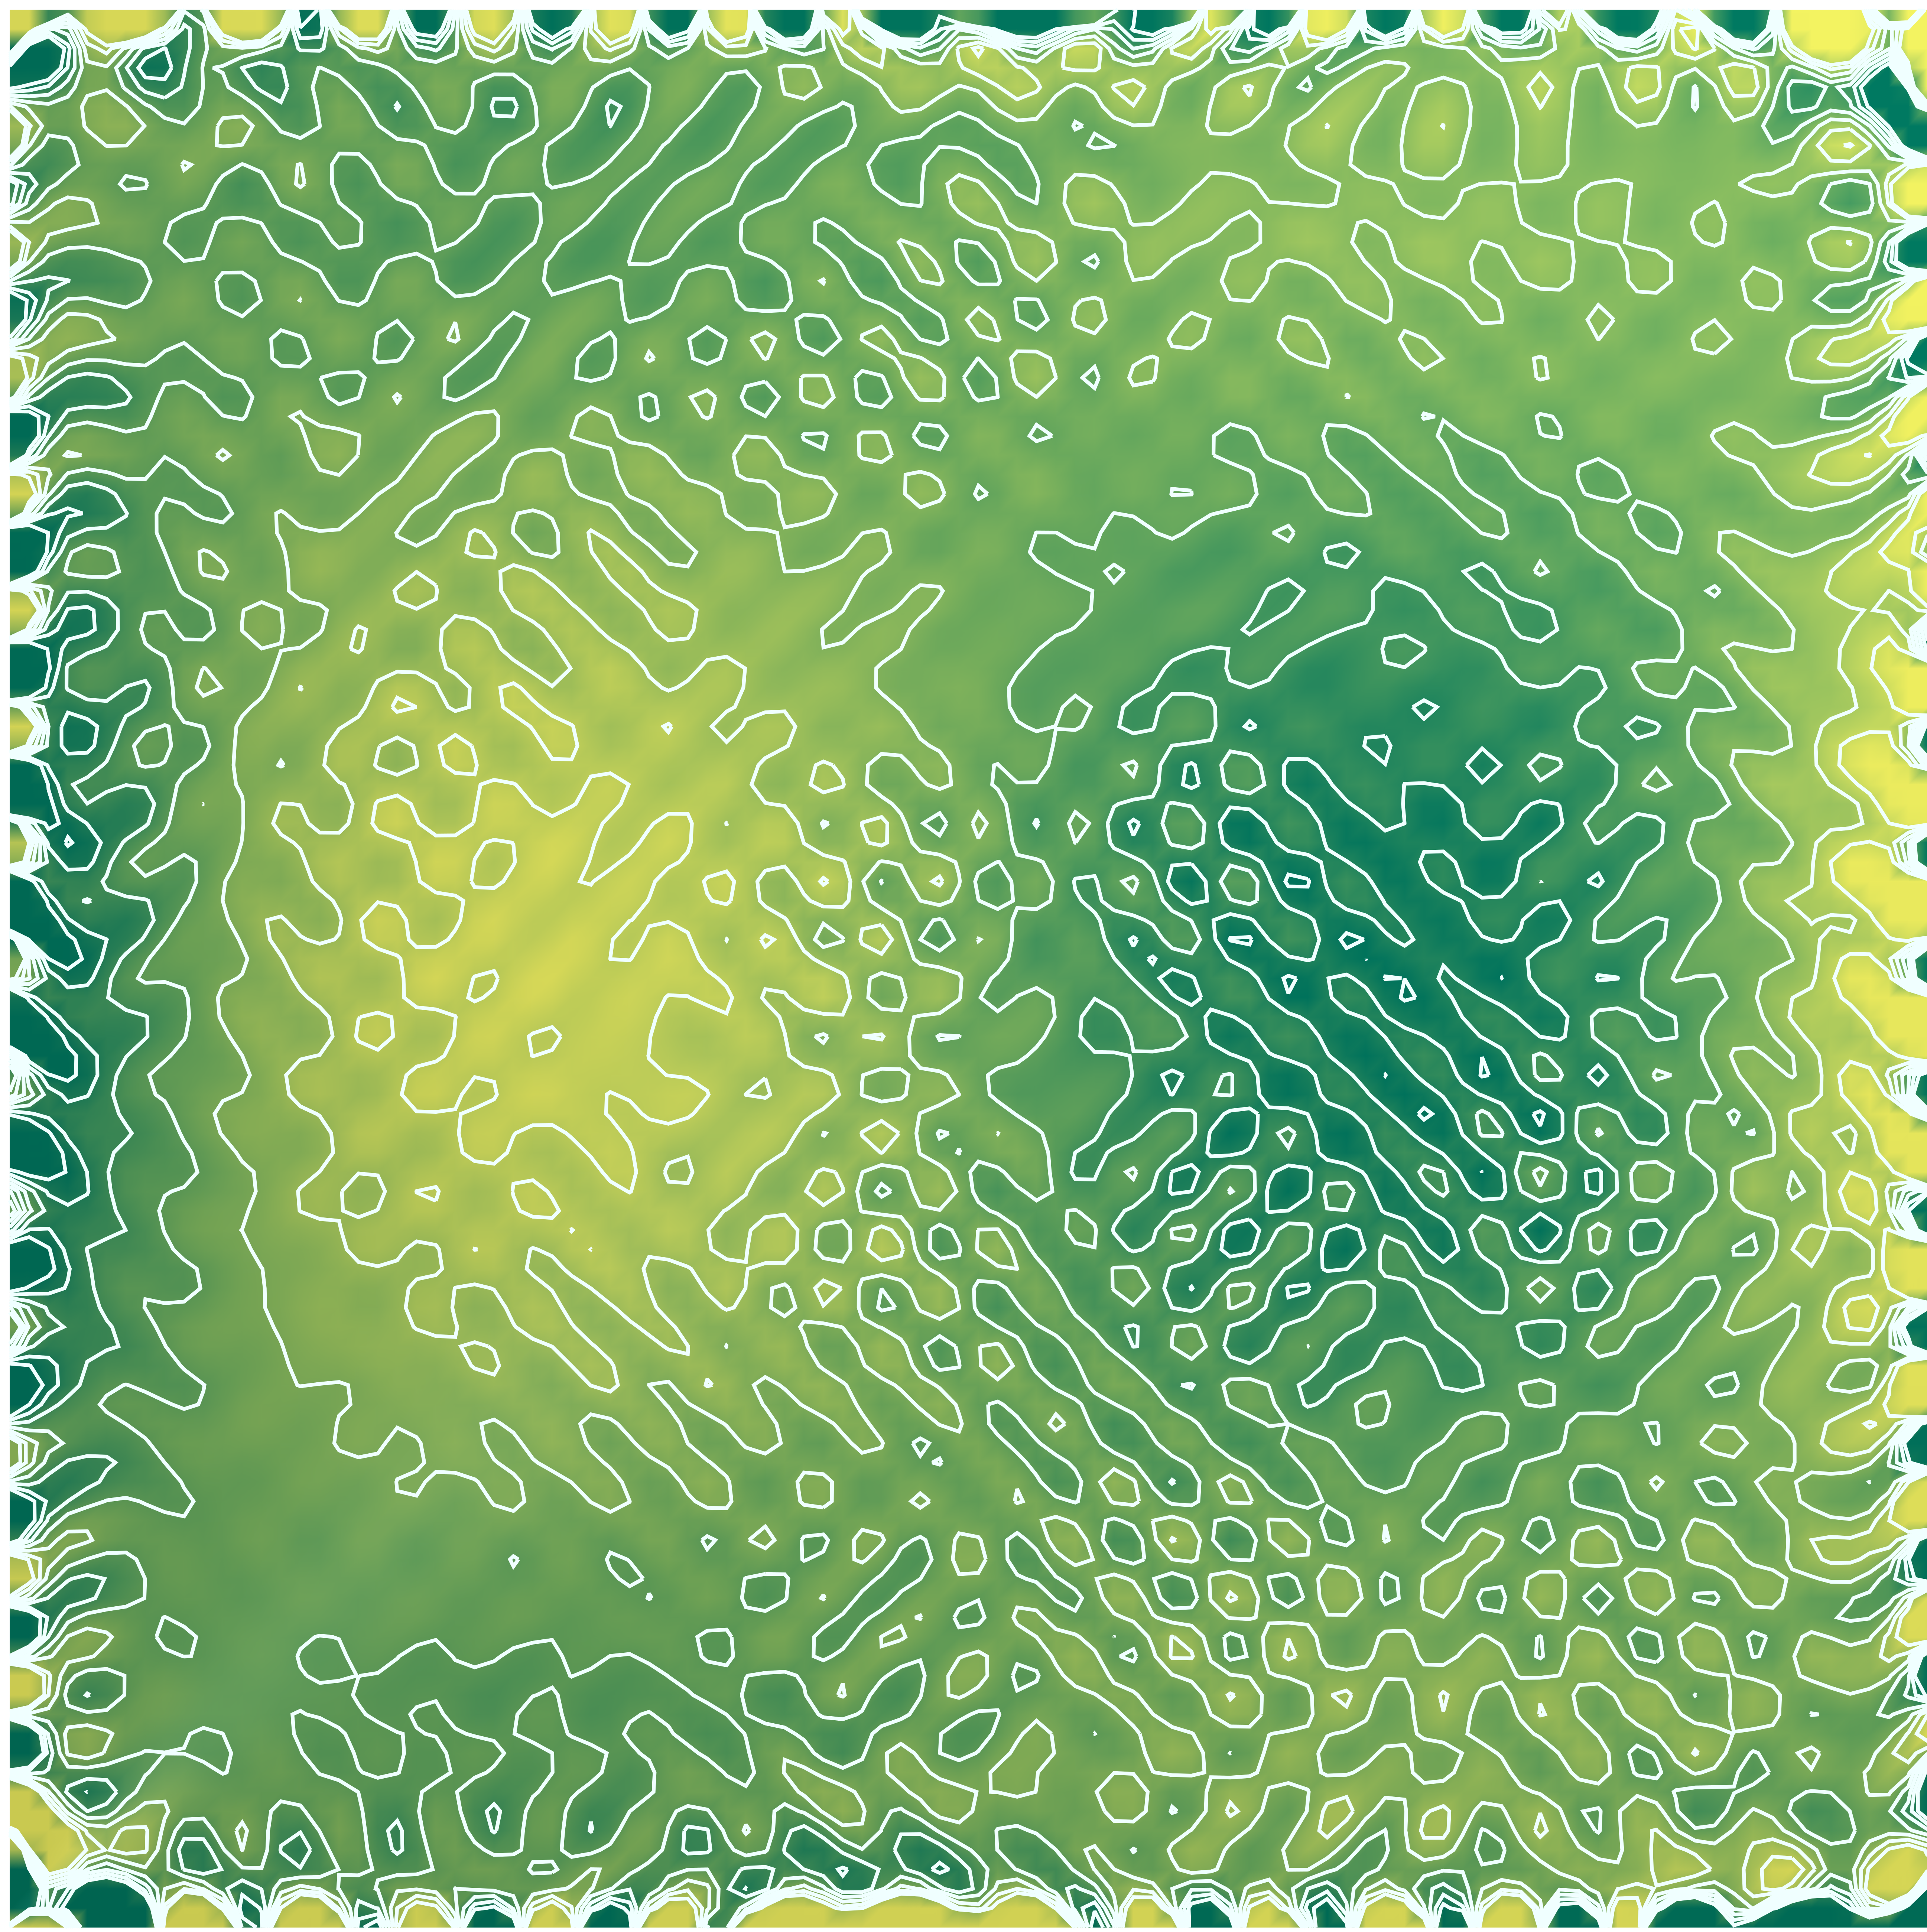
\includegraphics[width=0.4\textwidth]{figures/shearlocking/SquarePlate_mix_tri6_q1_16_16.png}}\end{subcaptiongroup}\\
    $4225$&\begin{subcaptiongroup}\raisebox{-0.5\height}{\includegraphics[width=0.4\textwidth]{figures/shearlocking/SquarePlate_mix_tri6_q1_32_25.png}}\end{subcaptiongroup}
    &\begin{subcaptiongroup}\raisebox{-0.5\height}{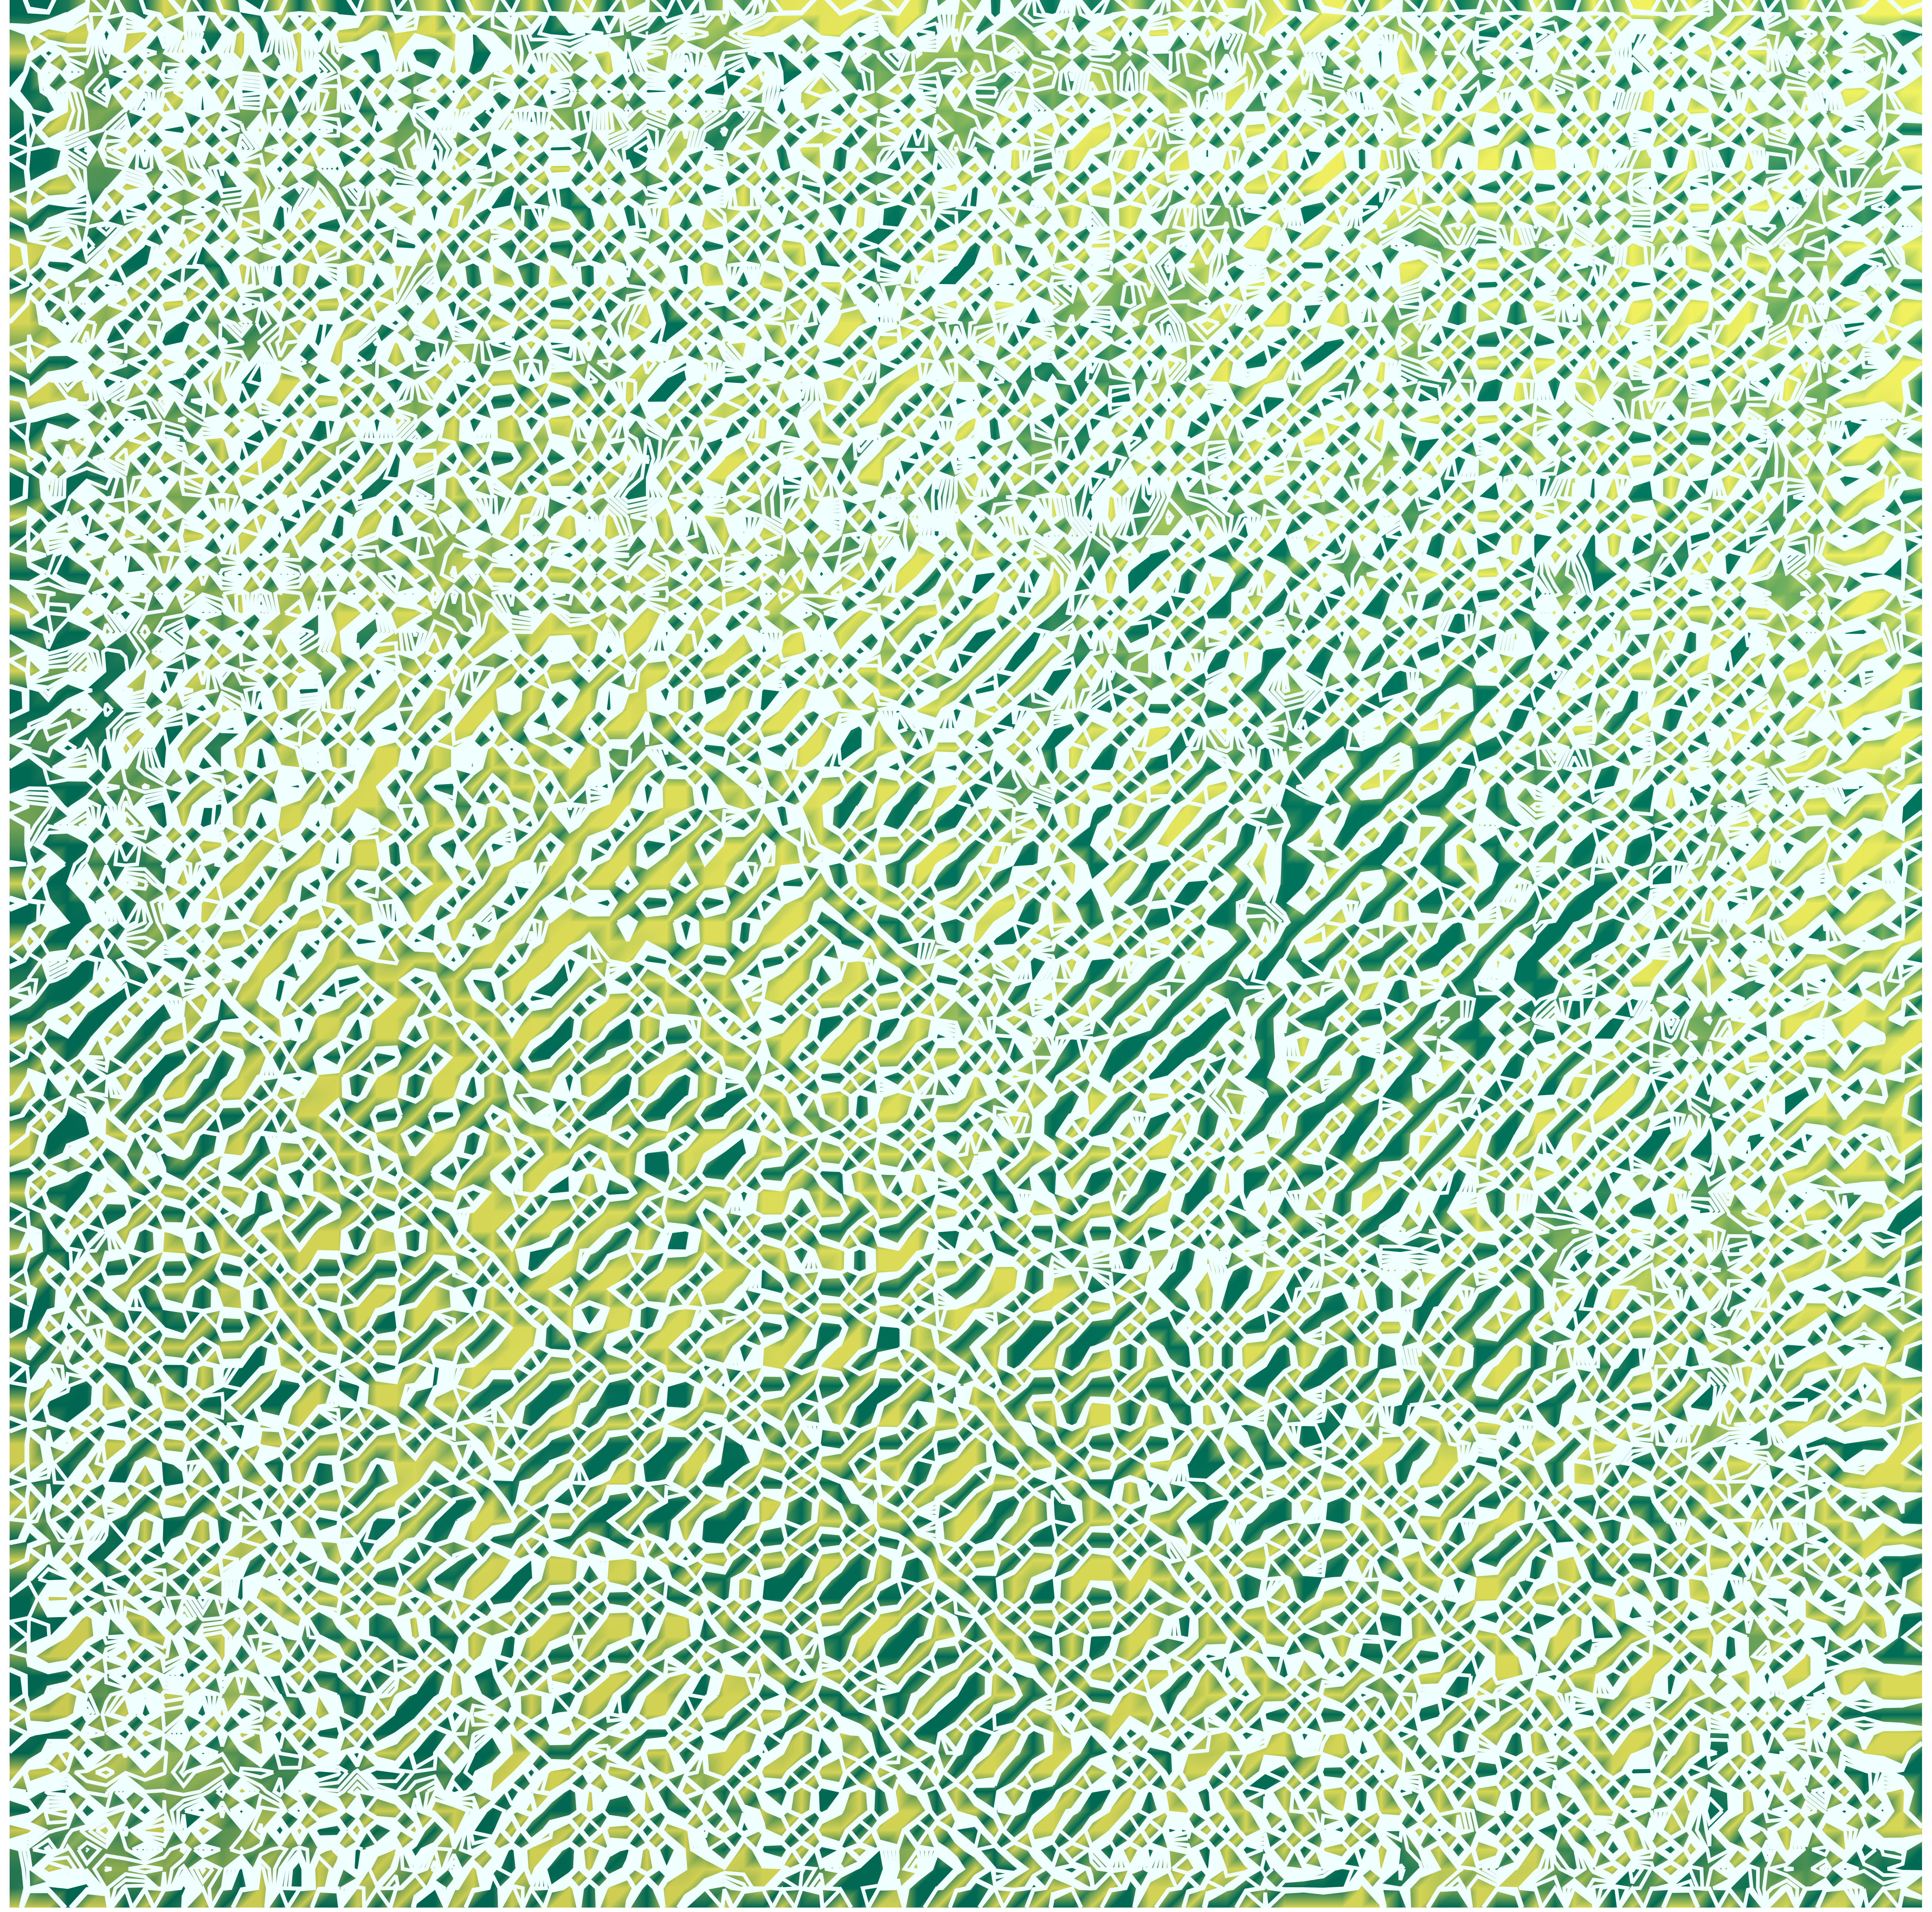
\includegraphics[width=0.4\textwidth]{figures/shearlocking/SquarePlate_mix_tri6_q1_32_32.png}}\end{subcaptiongroup}\\  
    \end{tabular}
    \caption{\textbf{固支方板问题Tri6单元应力云图($Q_1$)}}\label{Q1-Tri6}
\end{figure}

\begin{figure}[H]
    \centering
    \begin{tabular}{cccc}
    $\quad$&最优约束比&传统约束比\\
    $225$&\begin{subcaptiongroup}\raisebox{-0.4\height}{\includegraphics[width=0.4\textwidth]{figures/shearlocking/SquarePlate_mix_quad8_q1_8_6.png}}\end{subcaptiongroup}
    &\begin{subcaptiongroup}\raisebox{-0.4\height}{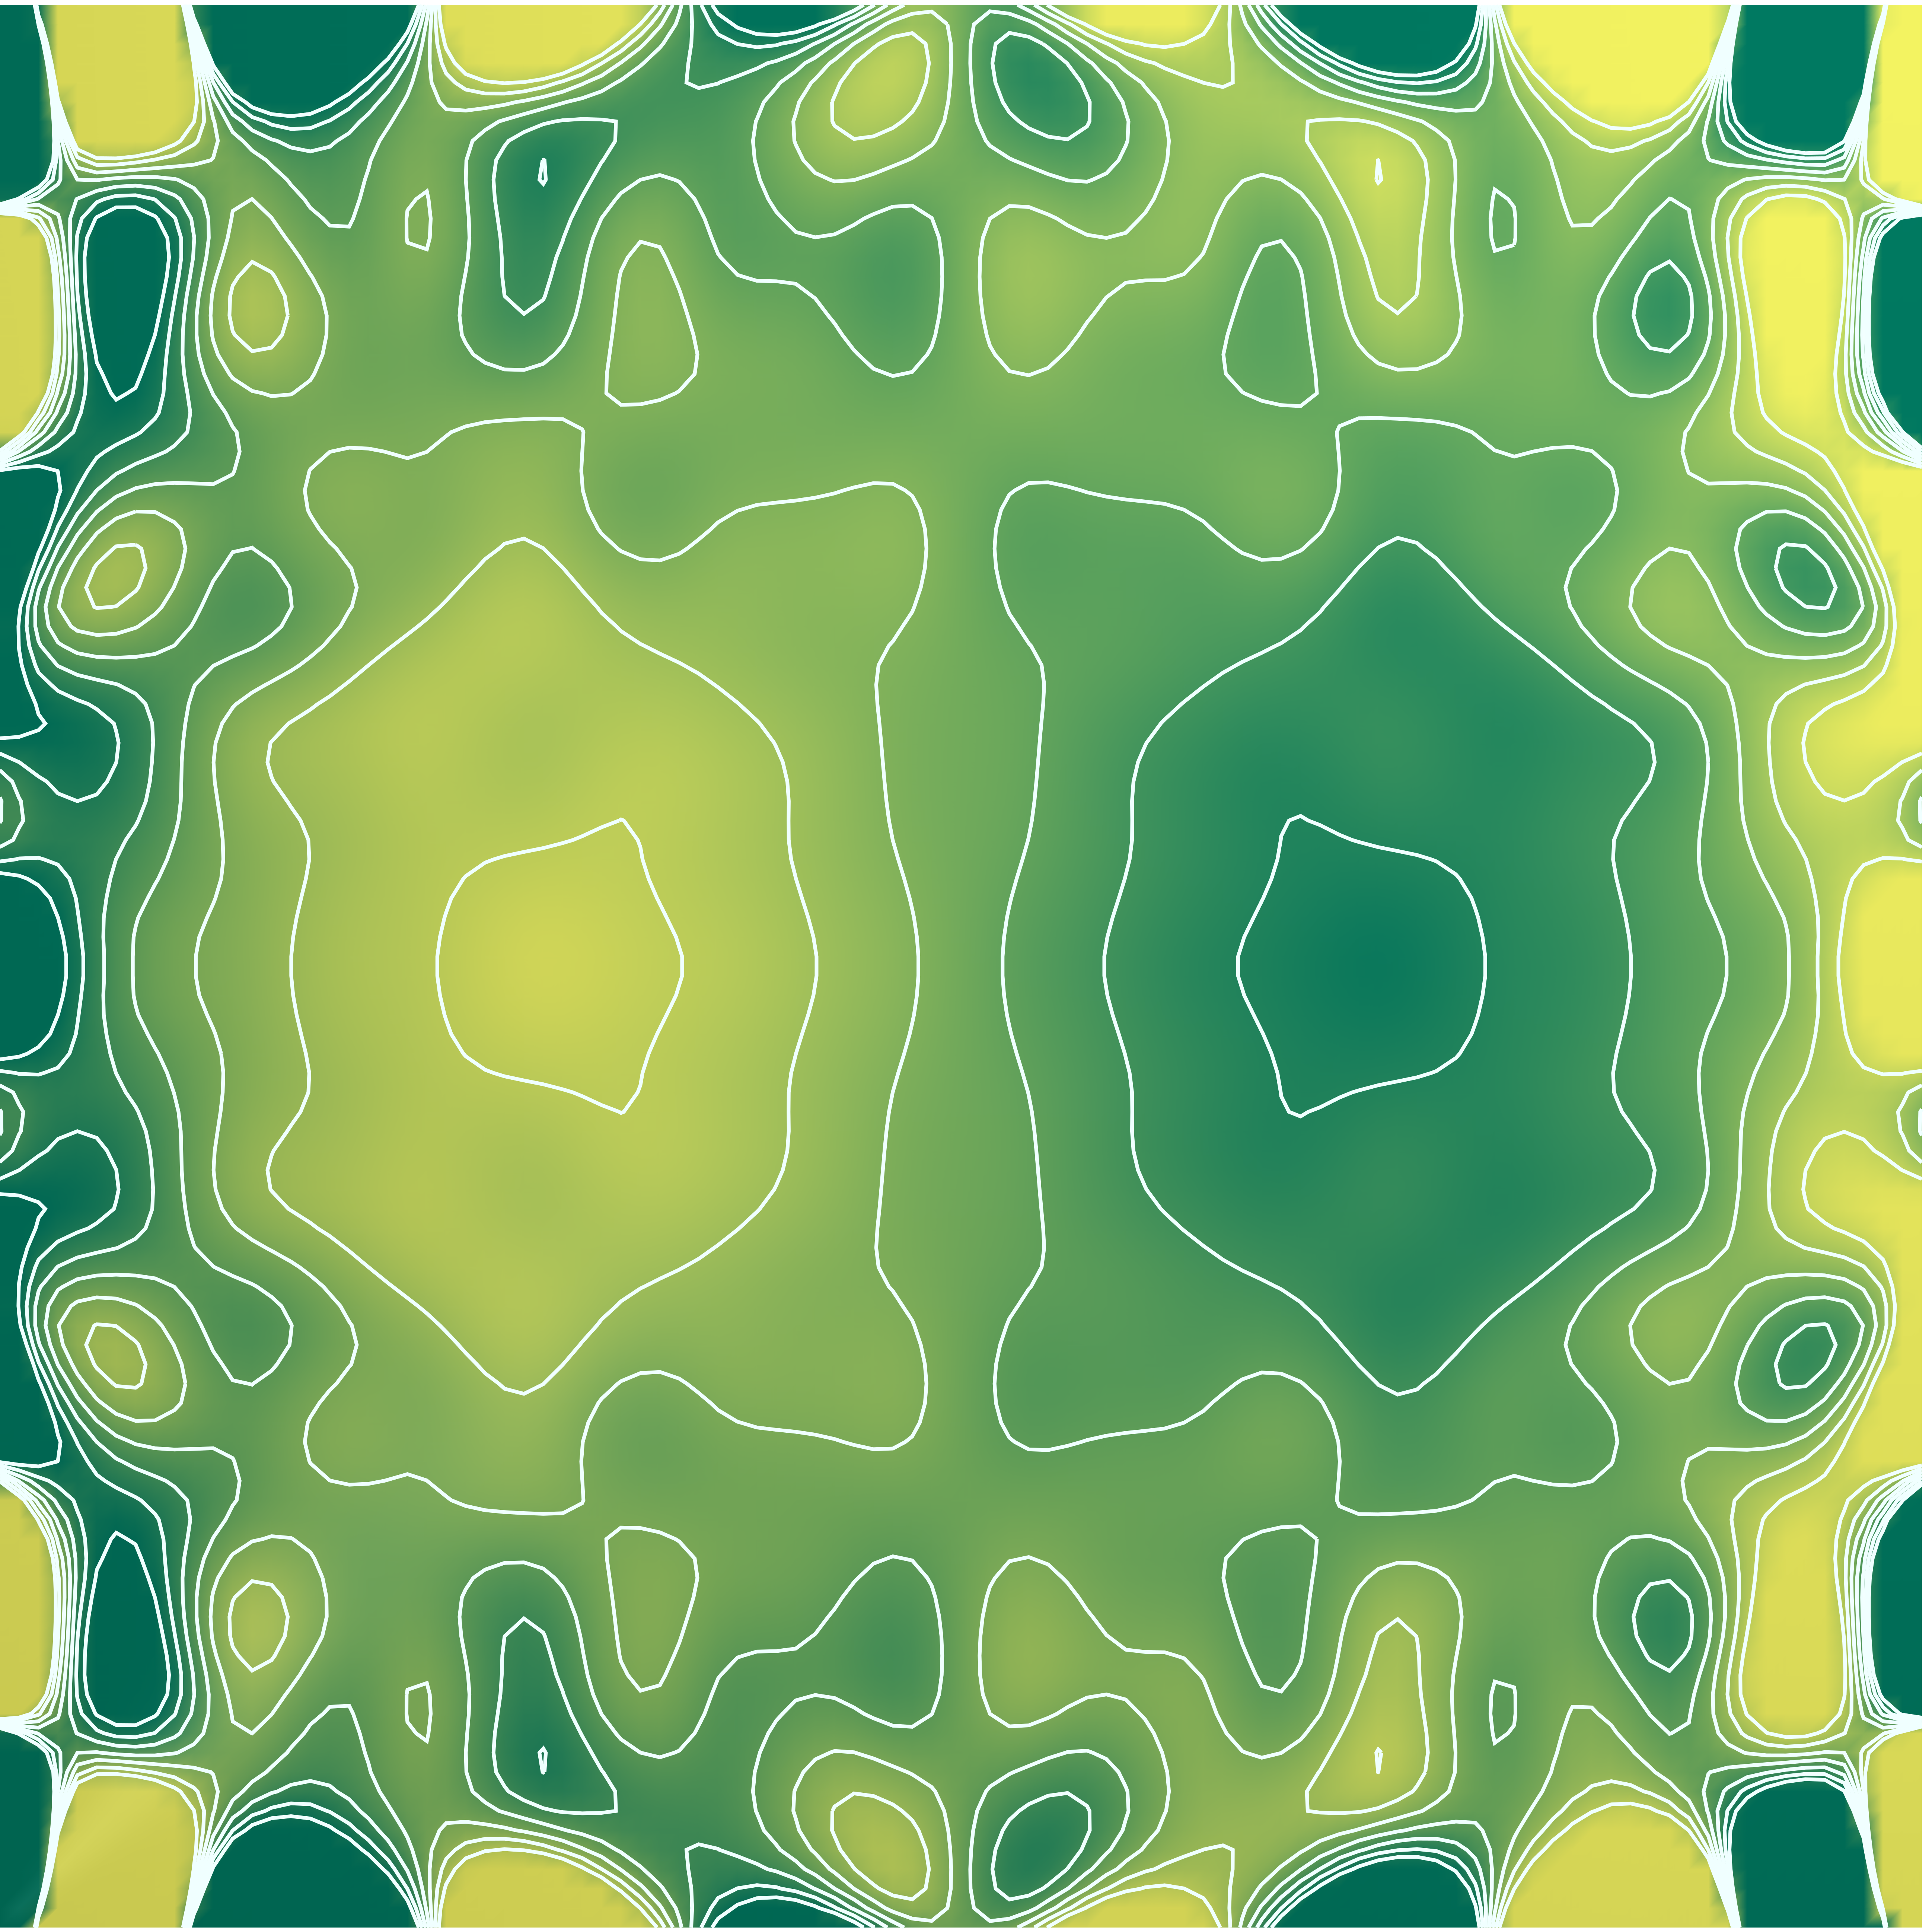
\includegraphics[width=0.4\textwidth]{figures/shearlocking/SquarePlate_mix_quad8_q1_8_8.png}}\end{subcaptiongroup}\\
    $833$&\begin{subcaptiongroup}\raisebox{-0.4\height}{\includegraphics[width=0.4\textwidth]{figures/shearlocking/SquarePlate_mix_quad8_q1_16_14.png}}\end{subcaptiongroup}
    &\begin{subcaptiongroup}\raisebox{-0.4\height}{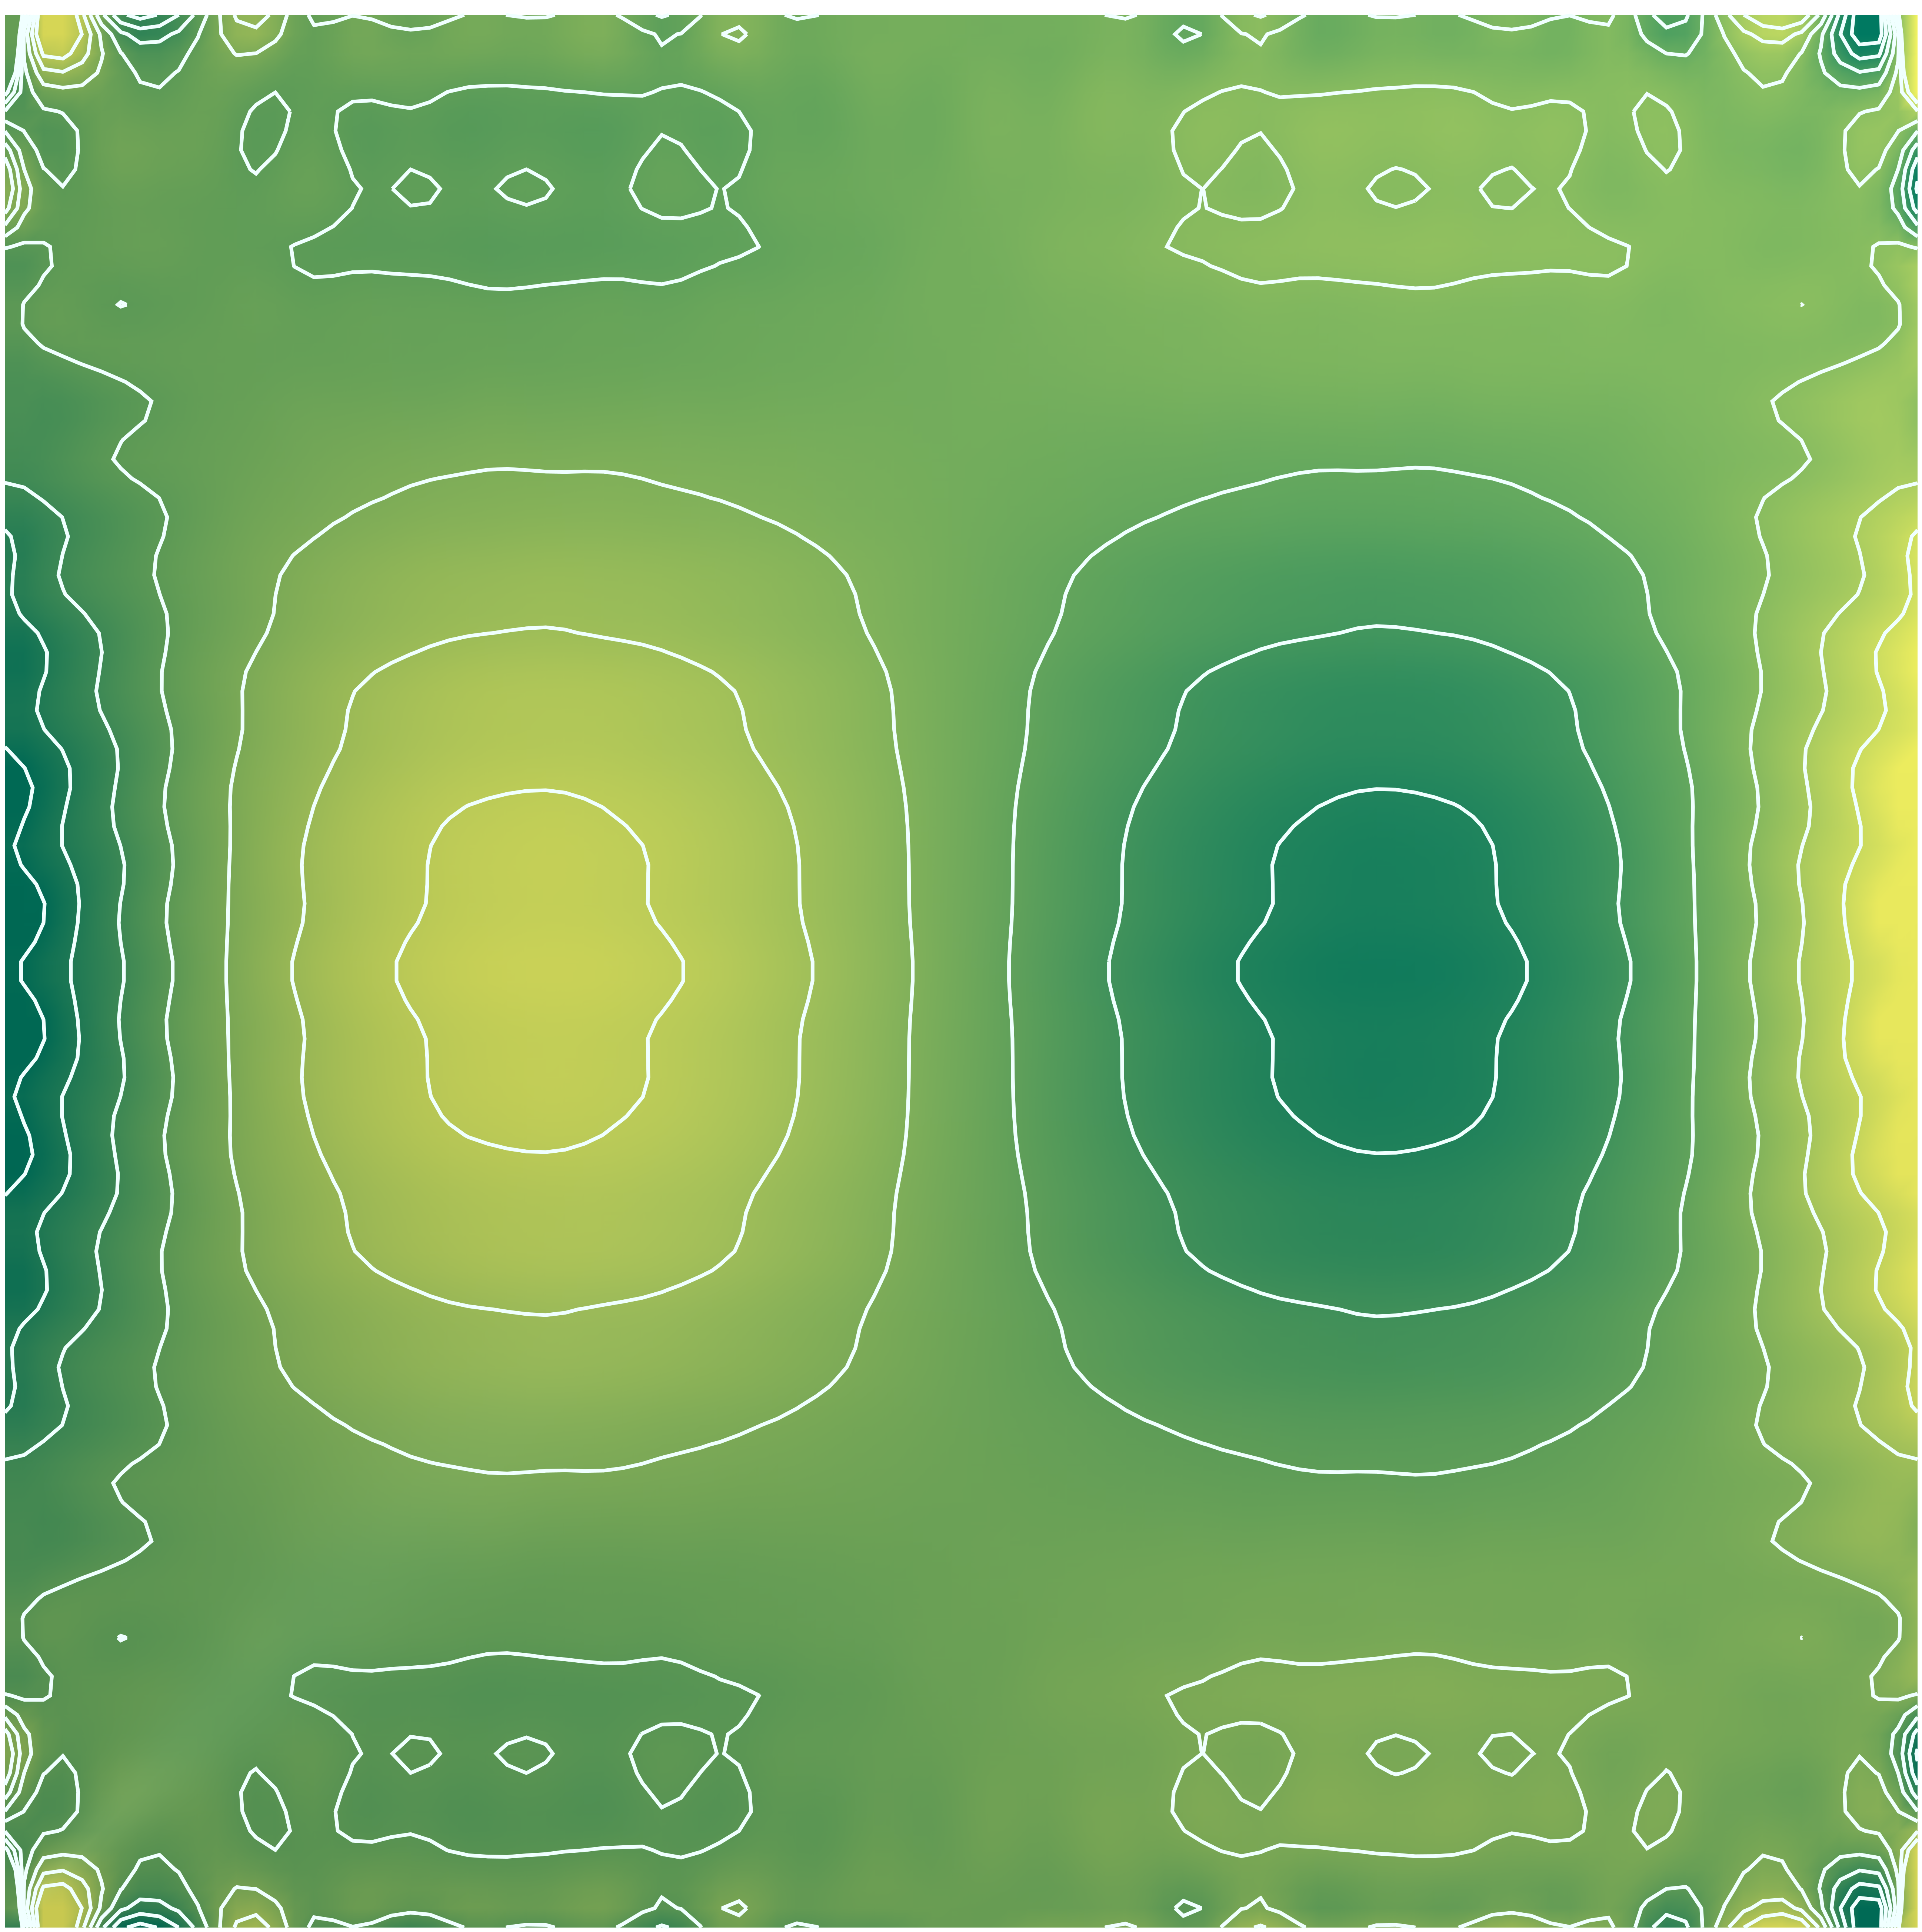
\includegraphics[width=0.4\textwidth]{figures/shearlocking/SquarePlate_mix_quad8_q1_16_16.png}}\end{subcaptiongroup}\\
    $3201$&\begin{subcaptiongroup}\raisebox{-0.4\height}{\includegraphics[width=0.4\textwidth]{figures/shearlocking/SquarePlate_mix_quad8_q1_32_26.png}}\end{subcaptiongroup}
    &\begin{subcaptiongroup}\raisebox{-0.4\height}{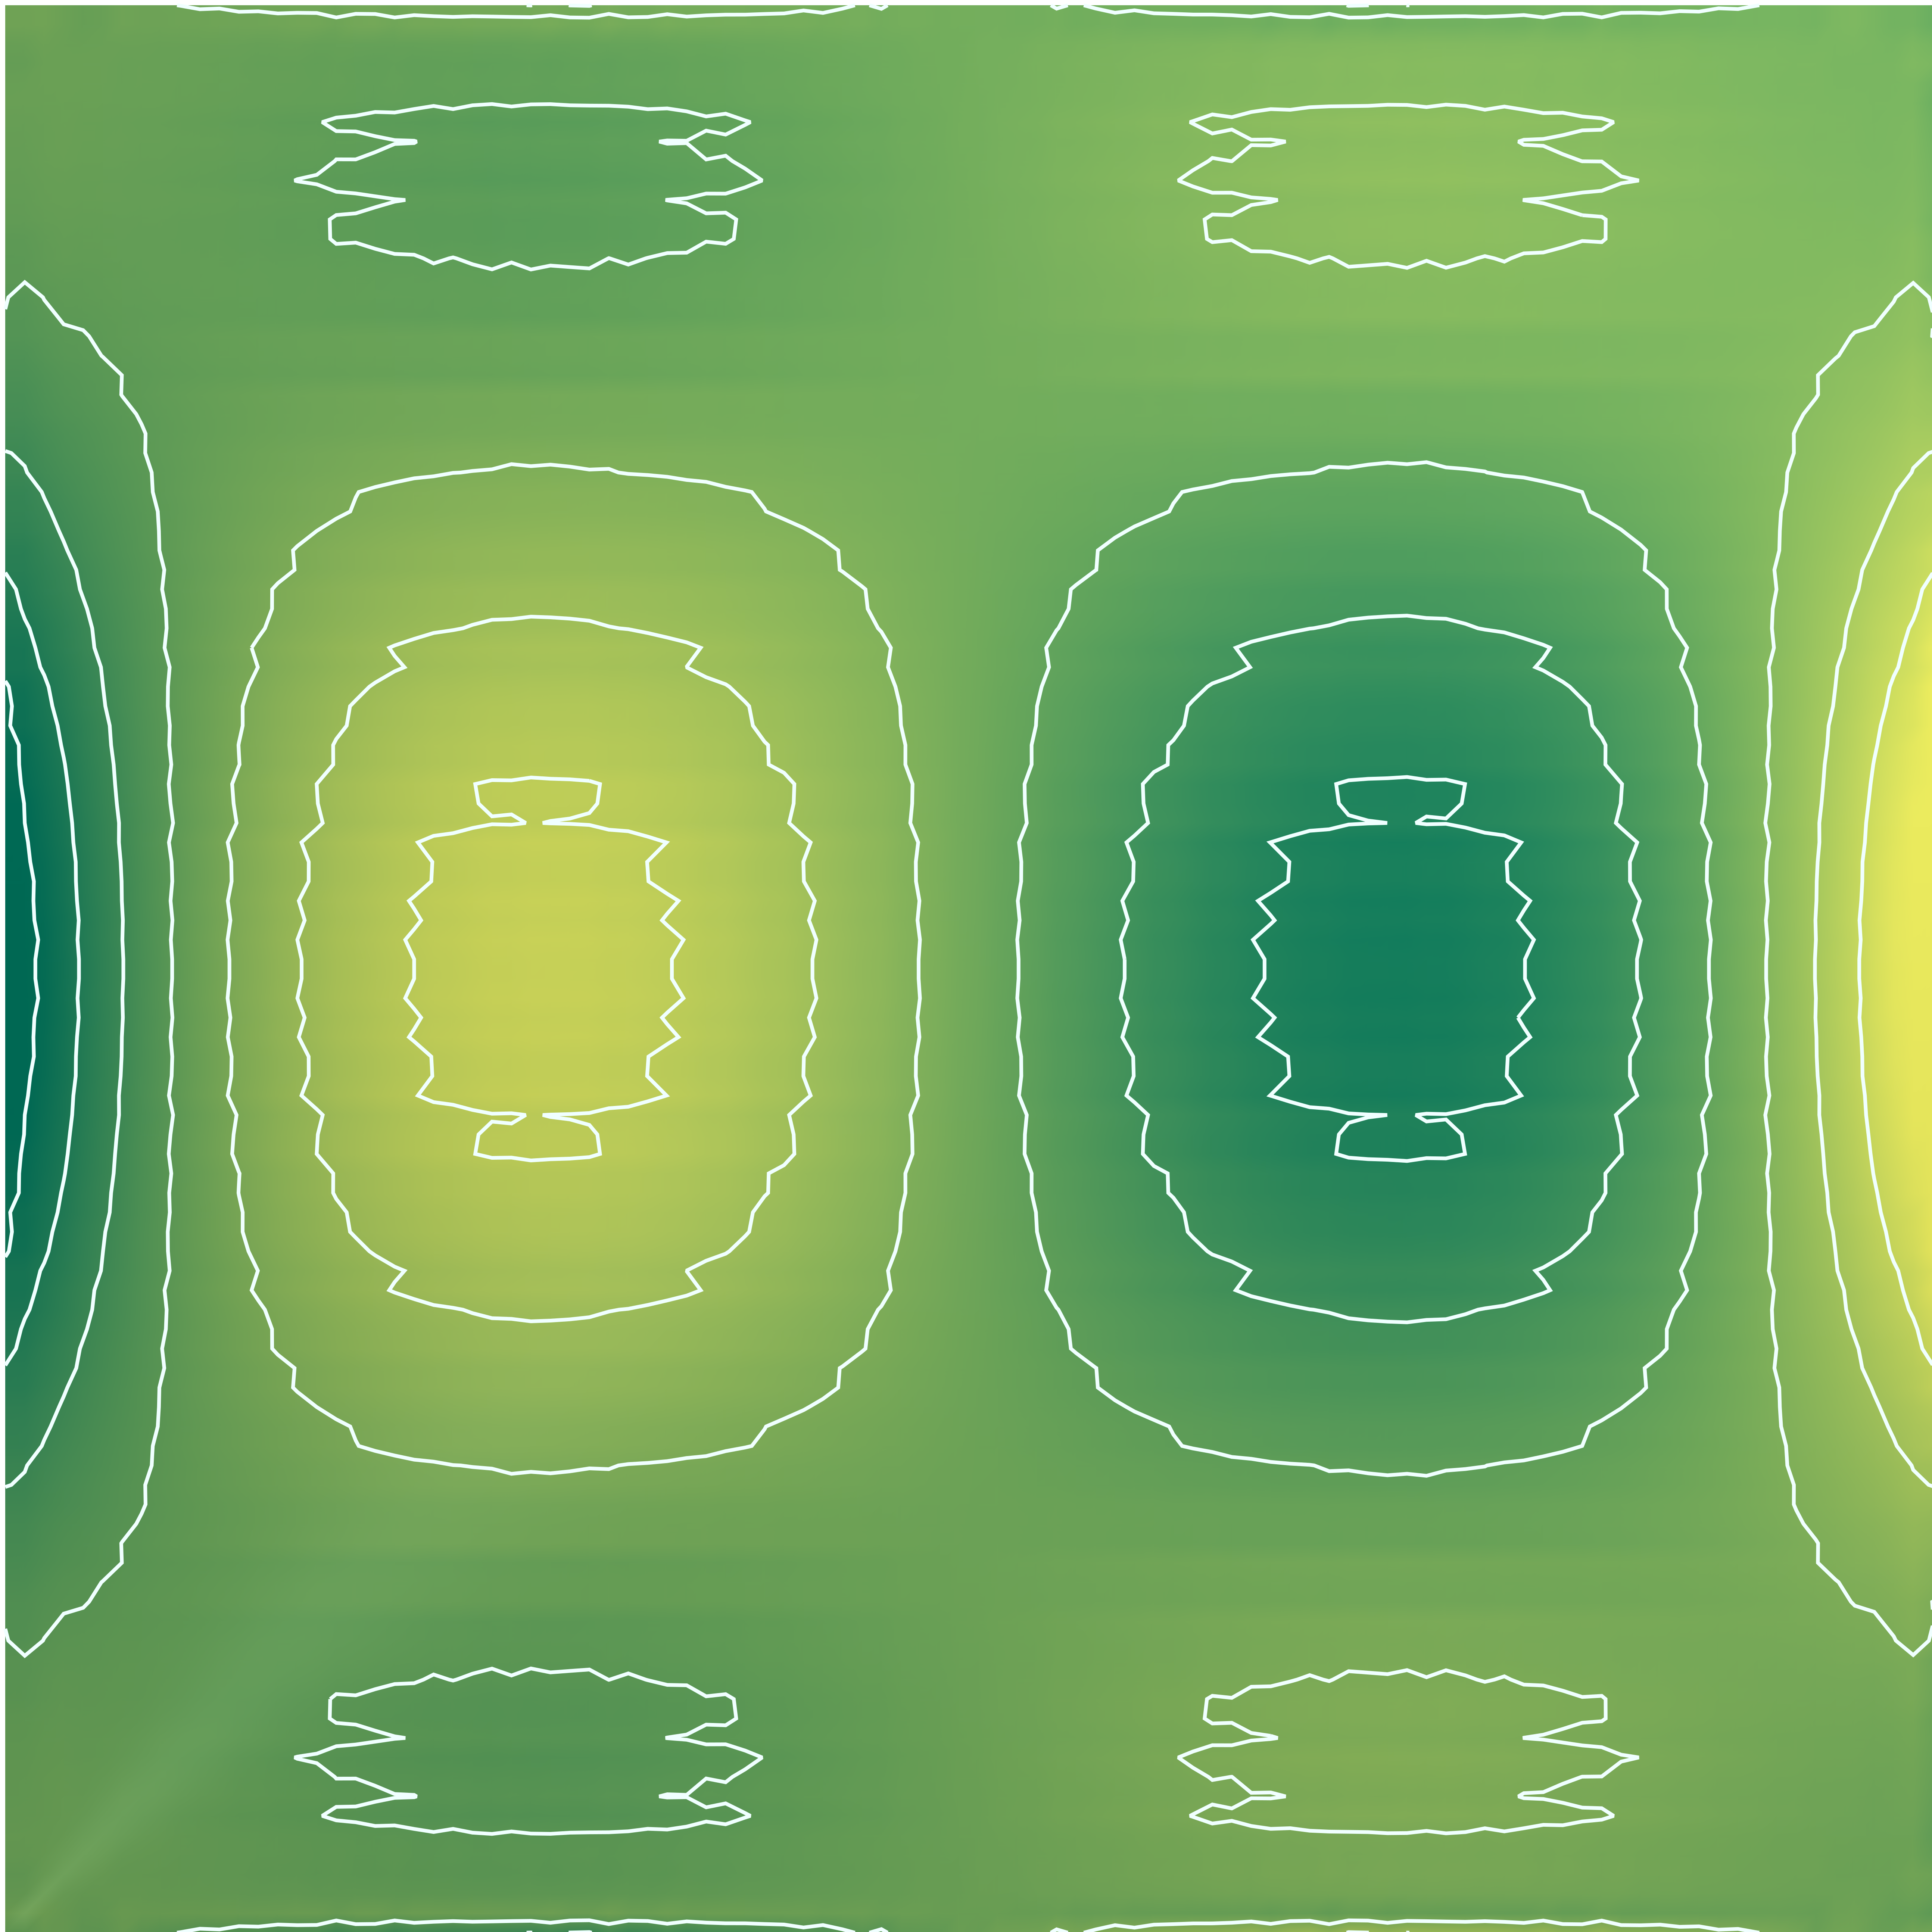
\includegraphics[width=0.4\textwidth]{figures/shearlocking/SquarePlate_mix_quad8_q1_32_32.png}}\end{subcaptiongroup}\\ 
    \end{tabular}
    \caption{\textbf{固支方板问题Quad8单元应力云图($Q_1$)}}\label{Q1-Quad8}
\end{figure}

\subsection{Razzaque斜板问题}
考虑如图\ref{xieplate}所示斜板问题,其中斜板的边长为$L=100$,厚度为$h=10,1,0.1$,均被荷载作用在板内为$\bar{q}=1$,材料系数分别为杨氏模量$E=1085$、泊松比$\nu=0.31$。该斜板中心位移$w_c$的参考解为:
\begin{equation} 
    \bar{w_c}=w_c\times10^2\frac{D}{\bar{q}L^4}
\end{equation}
如图\ref{xieplatemsh}所示,斜板求解域采用均布离散的81、289、1089、4225四个疏密不同的节点进行离散,同样采用线性单元和二次单元进行数值分析。
\begin{figure}[H]
    \centering 
        \includegraphics[scale=0.6]{figures/shearlocking/xie plate.png}
        \caption{Razzaque斜板问题模型}\label{xieplate}
\end{figure}
\begin{figure}[H]
    \centering 
        \includegraphics[scale=0.5]{figures/shearlocking/xieplatemsh.png}
        \caption{Razzaque斜板问题模型}\label{xieplatemsh}
\end{figure}
\begin{figure}[H]
    \centering
    \begin{tabular}{cccc}
    $\quad$&最优约束比&传统约束比\\
    $81$&\begin{subcaptiongroup}\raisebox{-0.4\height}{\includegraphics[width=0.4\textwidth]{figures/shearlocking/MorleysAcuteSkewPlate_tri3_q1_8_6.png}}\end{subcaptiongroup}
    &\begin{subcaptiongroup}\raisebox{-0.4\height}{\includegraphics[width=0.4\textwidth]{figures/shearlocking/MorleysAcuteSkewPlate_tri3_q1_8_8.png}}\end{subcaptiongroup}\\ 
    $289$&\begin{subcaptiongroup}\raisebox{-0.4\height}{\includegraphics[width=0.4\textwidth]{figures/shearlocking/MorleysAcuteSkewPlate_tri3_q1_16_12.png}}\end{subcaptiongroup}
    &\begin{subcaptiongroup}\raisebox{-0.4\height}{\includegraphics[width=0.4\textwidth]{figures/shearlocking/MorleysAcuteSkewPlate_tri3_q1_16_16.png}}\end{subcaptiongroup}\\ 
    $1089$&\begin{subcaptiongroup}\raisebox{-0.4\height}{\includegraphics[width=0.4\textwidth]{figures/shearlocking/MorleysAcuteSkewPlate_tri3_q1_32_26.png}}\end{subcaptiongroup}
    &\begin{subcaptiongroup}\raisebox{-0.4\height}{\includegraphics[width=0.4\textwidth]{figures/shearlocking/MorleysAcuteSkewPlate_tri3_q1_32_32.png}}\end{subcaptiongroup}\\ 
    \end{tabular}
    \caption{\textbf{Razzaque斜板问题Tri3单元应力云图($Q_1$)}}\label{XQ1-Tri3}
\end{figure}
\begin{figure}[H]
    \centering
    \begin{tabular}{cccc}
    $\quad$&最优约束比&传统约束比\\
    $81$&\begin{subcaptiongroup}\raisebox{-0.4\height}{\includegraphics[width=0.4\textwidth]{figures/shearlocking/MorleysAcuteSkewPlate_quad4_q1_8_6.png}}\end{subcaptiongroup}
    &\begin{subcaptiongroup}\raisebox{-0.4\height}{\includegraphics[width=0.4\textwidth]{figures/shearlocking/MorleysAcuteSkewPlate_quad4_q1_8_8.png}}\end{subcaptiongroup}\\ 
    $289$&\begin{subcaptiongroup}\raisebox{-0.4\height}{\includegraphics[width=0.4\textwidth]{figures/shearlocking/MorleysAcuteSkewPlate_quad4_q1_16_12.png}}\end{subcaptiongroup}
    &\begin{subcaptiongroup}\raisebox{-0.4\height}{\includegraphics[width=0.4\textwidth]{figures/shearlocking/MorleysAcuteSkewPlate_quad4_q1_16_16.png}}\end{subcaptiongroup}\\ 
    $1089$&\begin{subcaptiongroup}\raisebox{-0.4\height}{\includegraphics[width=0.4\textwidth]{figures/shearlocking/MorleysAcuteSkewPlate_quad4_q1_32_26.png}}\end{subcaptiongroup}
    &\begin{subcaptiongroup}\raisebox{-0.4\height}{\includegraphics[width=0.4\textwidth]{figures/shearlocking/MorleysAcuteSkewPlate_quad4_q1_32_32.png}}\end{subcaptiongroup}\\ 
    \end{tabular}
    \caption{\textbf{Razzaque斜板问题Quad4单元应力云图($Q_1$)}}\label{XQ1-Quad4}
\end{figure}
\begin{figure}[H]
    \centering
    \begin{tabular}{cccc}
    $\quad$&最优约束比&传统约束比\\
    $289$&\begin{subcaptiongroup}\raisebox{-0.4\height}{\includegraphics[width=0.4\textwidth]{figures/shearlocking/MorleysAcuteSkewPlate_tri6_q1_8_6.png}}\end{subcaptiongroup}
    &\begin{subcaptiongroup}\raisebox{-0.4\height}{\includegraphics[width=0.4\textwidth]{figures/shearlocking/MorleysAcuteSkewPlate_tri6_q1_8_8.png}}\end{subcaptiongroup}\\ 
    $833$&\begin{subcaptiongroup}\raisebox{-0.4\height}{\includegraphics[width=0.4\textwidth]{figures/shearlocking/MorleysAcuteSkewPlate_tri6_q1_16_12.png}}\end{subcaptiongroup}
    &\begin{subcaptiongroup}\raisebox{-0.4\height}{\includegraphics[width=0.4\textwidth]{figures/shearlocking/MorleysAcuteSkewPlate_tri6_q1_16_16.png}}\end{subcaptiongroup}\\ 
    $4225$&\begin{subcaptiongroup}\raisebox{-0.4\height}{\includegraphics[width=0.4\textwidth]{figures/shearlocking/MorleysAcuteSkewPlate_tri6_q1_32_26.png}}\end{subcaptiongroup}
    &\begin{subcaptiongroup}\raisebox{-0.4\height}{\includegraphics[width=0.4\textwidth]{figures/shearlocking/MorleysAcuteSkewPlate_tri6_q1_32_32.png}}\end{subcaptiongroup}\\ 
    \end{tabular}
    \caption{\textbf{Razzaque斜板问题Tri6单元应力云图($Q_1$)}}
    % \label{XQ1-Tri6}
\end{figure}
\begin{figure}[H]
    \centering
    \begin{tabular}{cccc}
    $\quad$&最优约束比&传统约束比\\
    $225$&\begin{subcaptiongroup}\raisebox{-0.4\height}{\includegraphics[width=0.4\textwidth]{figures/shearlocking/MorleysAcuteSkewPlate_quad8_q1_8_6.png}}\end{subcaptiongroup}
    &\begin{subcaptiongroup}\raisebox{-0.4\height}{\includegraphics[width=0.4\textwidth]{figures/shearlocking/MorleysAcuteSkewPlate_quad8_q1_8_8.png}}\end{subcaptiongroup}\\ 
    $833$&\begin{subcaptiongroup}\raisebox{-0.4\height}{\includegraphics[width=0.4\textwidth]{figures/shearlocking/MorleysAcuteSkewPlate_quad8_q1_16_12.png}}\end{subcaptiongroup}
    &\begin{subcaptiongroup}\raisebox{-0.4\height}{\includegraphics[width=0.4\textwidth]{figures/shearlocking/MorleysAcuteSkewPlate_quad8_q1_16_16.png}}\end{subcaptiongroup}\\ 
    $3201$&\begin{subcaptiongroup}\raisebox{-0.4\height}{\includegraphics[width=0.4\textwidth]{figures/shearlocking/MorleysAcuteSkewPlate_quad8_q1_32_26.png}}\end{subcaptiongroup}
    &\begin{subcaptiongroup}\raisebox{-0.4\height}{\includegraphics[width=0.4\textwidth]{figures/shearlocking/MorleysAcuteSkewPlate_quad8_q1_32_32.png}}\end{subcaptiongroup}\\ 
    \end{tabular}
    \caption{\textbf{Razzaque斜板问题Quad8单元应力云图($Q_1$)}}\label{XQ1-Tri6}
\end{figure}
\subsection{简支圆板问题}
考虑如图\ref{yuanplate}所示简支圆板问题,其中圆板的半径为$R=5$,均匀荷载作用在板内为$\bar{q}=1$,材料系数分别为杨氏模量$E=10.92$、泊松比$\nu=0.3$。该圆板板中心位移$w_c$的精确解与板厚具有以下关系:

\begin{table} 
    \centering
    \caption{均匀荷载下简支圆板中心位移$w_c$}
    \begin{tabular}{l|c|r}
        \hline
        0.1   &1      & 2.5   \\
        39831 &41.599 & 3.262 \\
        \hline
    \end{tabular}
\end{table}
如图\ref{yuanplatemsh}所示,圆板求解域采用均布离散的61、217、817、3169四个疏密不同的节点进行离散,同样采用线性单元和二次单元进行数值分析。
\begin{figure}[H]
    \centering 
        \includegraphics[scale=0.8]{figures/shearlocking/yuan plate.png}
        \caption{简支圆板问题模型}\label{yuanplate}
\end{figure}22
\begin{figure}[H]
    \centering 
        \includegraphics[scale=0.5]{figures/shearlocking/yuanplatemsh.png}
        \caption{简支圆板问题节点离散}\label{yuanplatemsh}
\end{figure}
\begin{figure}[H]
    \centering
    \begin{tabular}{cccc}
    $\quad$&最优约束比&传统约束比\\
    $61$&\begin{subcaptiongroup}\raisebox{-0.4\height}{\includegraphics[width=0.4\textwidth]{figures/shearlocking/Circular_tri3_q1_8_6.png}}\end{subcaptiongroup}
    &\begin{subcaptiongroup}\raisebox{-0.4\height}{\includegraphics[width=0.4\textwidth]{figures/shearlocking/Circular_tri3_q1_8_8.png}}\end{subcaptiongroup}\\ 
    $217$&\begin{subcaptiongroup}\raisebox{-0.4\height}{\includegraphics[width=0.4\textwidth]{figures/shearlocking/Circular_tri3_q1_16_12.png}}\end{subcaptiongroup}
    &\begin{subcaptiongroup}\raisebox{-0.4\height}{\includegraphics[width=0.4\textwidth]{figures/shearlocking/Circular_tri3_q1_16_16.png}}\end{subcaptiongroup}\\ 
    $817$&\begin{subcaptiongroup}\raisebox{-0.4\height}{\includegraphics[width=0.4\textwidth]{figures/shearlocking/Circular_tri3_q1_32_26.png}}\end{subcaptiongroup}
    &\begin{subcaptiongroup}\raisebox{-0.4\height}{\includegraphics[width=0.4\textwidth]{figures/shearlocking/Circular_tri3_q1_32_32.png}}\end{subcaptiongroup}\\ 
    \end{tabular}
    \caption{\textbf{简支圆板问题Tri3单元应力云图($Q_1$)}}\label{YQ1-Tri3}
\end{figure}
\begin{figure}[H]
    \centering
    \begin{tabular}{cccc}
    $\quad$&最优约束比&传统约束比\\
    $61$&\begin{subcaptiongroup}\raisebox{-0.4\height}{\includegraphics[width=0.4\textwidth]{figures/shearlocking/Circular_quad4_q1_8_6.png}}\end{subcaptiongroup}
    &\begin{subcaptiongroup}\raisebox{-0.4\height}{\includegraphics[width=0.4\textwidth]{figures/shearlocking/Circular_quad4_q1_8_8.png}}\end{subcaptiongroup}\\ 
    $217$&\begin{subcaptiongroup}\raisebox{-0.4\height}{\includegraphics[width=0.4\textwidth]{figures/shearlocking/Circular_quad4_q1_16_12.png}}\end{subcaptiongroup}
    &\begin{subcaptiongroup}\raisebox{-0.4\height}{\includegraphics[width=0.4\textwidth]{figures/shearlocking/Circular_quad4_q1_16_16.png}}\end{subcaptiongroup}\\ 
    $817$&\begin{subcaptiongroup}\raisebox{-0.4\height}{\includegraphics[width=0.4\textwidth]{figures/shearlocking/Circular_quad4_q1_32_26.png}}\end{subcaptiongroup}
    &\begin{subcaptiongroup}\raisebox{-0.4\height}{\includegraphics[width=0.4\textwidth]{figures/shearlocking/Circular_quad4_q1_32_32.png}}\end{subcaptiongroup}\\ 
    \end{tabular}
    \caption{\textbf{简支圆板问题Quad4单元应力云图($Q_1$)}}\label{YQ1-Quad4}
\end{figure}
\begin{figure}[H]
    \centering
    \begin{tabular}{cccc}
    $\quad$&最优约束比&传统约束比\\
    $61$&\begin{subcaptiongroup}\raisebox{-0.4\height}{\includegraphics[width=0.4\textwidth]{figures/shearlocking/Circular_tri6_q1_8_6.png}}\end{subcaptiongroup}
    &\begin{subcaptiongroup}\raisebox{-0.4\height}{\includegraphics[width=0.4\textwidth]{figures/shearlocking/Circular_tri6_q1_8_8.png}}\end{subcaptiongroup}\\ 
    $217$&\begin{subcaptiongroup}\raisebox{-0.4\height}{\includegraphics[width=0.4\textwidth]{figures/shearlocking/Circular_tri6_q1_16_12.png}}\end{subcaptiongroup}
    &\begin{subcaptiongroup}\raisebox{-0.4\height}{\includegraphics[width=0.4\textwidth]{figures/shearlocking/Circular_tri6_q1_16_16.png}}\end{subcaptiongroup}\\ 
    $817$&\begin{subcaptiongroup}\raisebox{-0.4\height}{\includegraphics[width=0.4\textwidth]{figures/shearlocking/Circular_tri6_q1_32_26.png}}\end{subcaptiongroup}
    &\begin{subcaptiongroup}\raisebox{-0.4\height}{\includegraphics[width=0.4\textwidth]{figures/shearlocking/Circular_tri6_q1_32_32.png}}\end{subcaptiongroup}\\ 
    \end{tabular}
    \caption{\textbf{简支圆板问题Tri6单元应力云图($Q_1$)}}\label{YQ1-Tri6}
\end{figure}
\begin{figure}[H]
    \centering
    \begin{tabular}{cccc}
    $\quad$&最优约束比&传统约束比\\
    $61$&\begin{subcaptiongroup}\raisebox{-0.4\height}{\includegraphics[width=0.4\textwidth]{figures/shearlocking/Circular_quad8_q1_8_6.png}}\end{subcaptiongroup}
    &\begin{subcaptiongroup}\raisebox{-0.4\height}{\includegraphics[width=0.4\textwidth]{figures/shearlocking/Circular_quad8_q1_8_8.png}}\end{subcaptiongroup}\\ 
    $217$&\begin{subcaptiongroup}\raisebox{-0.4\height}{\includegraphics[width=0.4\textwidth]{figures/shearlocking/Circular_quad4_q1_16_12.png}}\end{subcaptiongroup}
    &\begin{subcaptiongroup}\raisebox{-0.4\height}{\includegraphics[width=0.4\textwidth]{figures/shearlocking/Circular_quad8_q1_16_16.png}}\end{subcaptiongroup}\\ 
    $817$&\begin{subcaptiongroup}\raisebox{-0.4\height}{\includegraphics[width=0.4\textwidth]{figures/shearlocking/Circular_quad4_q1_32_26.png}}\end{subcaptiongroup}
    &\begin{subcaptiongroup}\raisebox{-0.4\height}{\includegraphics[width=0.4\textwidth]{figures/shearlocking/Circular_quad8_q1_32_32.png}}\end{subcaptiongroup}\\ 
    \end{tabular}
    \caption{\textbf{简支圆板问题Quad8单元应力云图($Q_1$)}}\label{YQ1-Quad8}
\end{figure}